% Options for packages loaded elsewhere
\PassOptionsToPackage{unicode}{hyperref}
\PassOptionsToPackage{hyphens}{url}
%
\documentclass[
]{article}
\usepackage{lmodern}
\usepackage{amssymb,amsmath}
\usepackage{ifxetex,ifluatex}
\ifnum 0\ifxetex 1\fi\ifluatex 1\fi=0 % if pdftex
  \usepackage[T1]{fontenc}
  \usepackage[utf8]{inputenc}
  \usepackage{textcomp} % provide euro and other symbols
\else % if luatex or xetex
  \usepackage{unicode-math}
  \defaultfontfeatures{Scale=MatchLowercase}
  \defaultfontfeatures[\rmfamily]{Ligatures=TeX,Scale=1}
\fi
% Use upquote if available, for straight quotes in verbatim environments
\IfFileExists{upquote.sty}{\usepackage{upquote}}{}
\IfFileExists{microtype.sty}{% use microtype if available
  \usepackage[]{microtype}
  \UseMicrotypeSet[protrusion]{basicmath} % disable protrusion for tt fonts
}{}
\makeatletter
\@ifundefined{KOMAClassName}{% if non-KOMA class
  \IfFileExists{parskip.sty}{%
    \usepackage{parskip}
  }{% else
    \setlength{\parindent}{0pt}
    \setlength{\parskip}{6pt plus 2pt minus 1pt}}
}{% if KOMA class
  \KOMAoptions{parskip=half}}
\makeatother
\usepackage{xcolor}
\IfFileExists{xurl.sty}{\usepackage{xurl}}{} % add URL line breaks if available
\IfFileExists{bookmark.sty}{\usepackage{bookmark}}{\usepackage{hyperref}}
\hypersetup{
  pdftitle={final\_project\_markdown},
  pdfauthor={Eric Lyall},
  hidelinks,
  pdfcreator={LaTeX via pandoc}}
\urlstyle{same} % disable monospaced font for URLs
\usepackage[margin=1in]{geometry}
\usepackage{color}
\usepackage{fancyvrb}
\newcommand{\VerbBar}{|}
\newcommand{\VERB}{\Verb[commandchars=\\\{\}]}
\DefineVerbatimEnvironment{Highlighting}{Verbatim}{commandchars=\\\{\}}
% Add ',fontsize=\small' for more characters per line
\usepackage{framed}
\definecolor{shadecolor}{RGB}{248,248,248}
\newenvironment{Shaded}{\begin{snugshade}}{\end{snugshade}}
\newcommand{\AlertTok}[1]{\textcolor[rgb]{0.94,0.16,0.16}{#1}}
\newcommand{\AnnotationTok}[1]{\textcolor[rgb]{0.56,0.35,0.01}{\textbf{\textit{#1}}}}
\newcommand{\AttributeTok}[1]{\textcolor[rgb]{0.77,0.63,0.00}{#1}}
\newcommand{\BaseNTok}[1]{\textcolor[rgb]{0.00,0.00,0.81}{#1}}
\newcommand{\BuiltInTok}[1]{#1}
\newcommand{\CharTok}[1]{\textcolor[rgb]{0.31,0.60,0.02}{#1}}
\newcommand{\CommentTok}[1]{\textcolor[rgb]{0.56,0.35,0.01}{\textit{#1}}}
\newcommand{\CommentVarTok}[1]{\textcolor[rgb]{0.56,0.35,0.01}{\textbf{\textit{#1}}}}
\newcommand{\ConstantTok}[1]{\textcolor[rgb]{0.00,0.00,0.00}{#1}}
\newcommand{\ControlFlowTok}[1]{\textcolor[rgb]{0.13,0.29,0.53}{\textbf{#1}}}
\newcommand{\DataTypeTok}[1]{\textcolor[rgb]{0.13,0.29,0.53}{#1}}
\newcommand{\DecValTok}[1]{\textcolor[rgb]{0.00,0.00,0.81}{#1}}
\newcommand{\DocumentationTok}[1]{\textcolor[rgb]{0.56,0.35,0.01}{\textbf{\textit{#1}}}}
\newcommand{\ErrorTok}[1]{\textcolor[rgb]{0.64,0.00,0.00}{\textbf{#1}}}
\newcommand{\ExtensionTok}[1]{#1}
\newcommand{\FloatTok}[1]{\textcolor[rgb]{0.00,0.00,0.81}{#1}}
\newcommand{\FunctionTok}[1]{\textcolor[rgb]{0.00,0.00,0.00}{#1}}
\newcommand{\ImportTok}[1]{#1}
\newcommand{\InformationTok}[1]{\textcolor[rgb]{0.56,0.35,0.01}{\textbf{\textit{#1}}}}
\newcommand{\KeywordTok}[1]{\textcolor[rgb]{0.13,0.29,0.53}{\textbf{#1}}}
\newcommand{\NormalTok}[1]{#1}
\newcommand{\OperatorTok}[1]{\textcolor[rgb]{0.81,0.36,0.00}{\textbf{#1}}}
\newcommand{\OtherTok}[1]{\textcolor[rgb]{0.56,0.35,0.01}{#1}}
\newcommand{\PreprocessorTok}[1]{\textcolor[rgb]{0.56,0.35,0.01}{\textit{#1}}}
\newcommand{\RegionMarkerTok}[1]{#1}
\newcommand{\SpecialCharTok}[1]{\textcolor[rgb]{0.00,0.00,0.00}{#1}}
\newcommand{\SpecialStringTok}[1]{\textcolor[rgb]{0.31,0.60,0.02}{#1}}
\newcommand{\StringTok}[1]{\textcolor[rgb]{0.31,0.60,0.02}{#1}}
\newcommand{\VariableTok}[1]{\textcolor[rgb]{0.00,0.00,0.00}{#1}}
\newcommand{\VerbatimStringTok}[1]{\textcolor[rgb]{0.31,0.60,0.02}{#1}}
\newcommand{\WarningTok}[1]{\textcolor[rgb]{0.56,0.35,0.01}{\textbf{\textit{#1}}}}
\usepackage{graphicx,grffile}
\makeatletter
\def\maxwidth{\ifdim\Gin@nat@width>\linewidth\linewidth\else\Gin@nat@width\fi}
\def\maxheight{\ifdim\Gin@nat@height>\textheight\textheight\else\Gin@nat@height\fi}
\makeatother
% Scale images if necessary, so that they will not overflow the page
% margins by default, and it is still possible to overwrite the defaults
% using explicit options in \includegraphics[width, height, ...]{}
\setkeys{Gin}{width=\maxwidth,height=\maxheight,keepaspectratio}
% Set default figure placement to htbp
\makeatletter
\def\fps@figure{htbp}
\makeatother
\setlength{\emergencystretch}{3em} % prevent overfull lines
\providecommand{\tightlist}{%
  \setlength{\itemsep}{0pt}\setlength{\parskip}{0pt}}
\setcounter{secnumdepth}{-\maxdimen} % remove section numbering

\title{final\_project\_markdown}
\author{Eric Lyall}
\date{2022-03-27}

\begin{document}
\maketitle

\#Introdution (Eric is writing this) The paper we are reviewing is
called ``Experimental evolution for niche breadth in bacteriophage T4
highlights the importance of structural genes''. It was the doctoral
thesis for Jenny Pham at the Department of Organismic and Evolutionary
Biology at Harvard University.. This paper anayzed the evolution of T4
bacteriophage, which is a lytic virus that infects E.coli. The purpose
of this paper was to gain a better understanding of ``niche breadth
evolution''. Researchers wanted to understand how growing T4
bacteiophage in different niches (different E.coli strains) drives
evolution. Specifically, this paper looked at what kind of genes were
likely to mutate, and how the niche influence mutations.

Methods: The authors grew T4 bacteriophage (derived from a common
ancestor) in 15 cultures of bacteria for approximately 50 generations.
Each culture was passages daily. 5 of the bacteria cultures had E.coli
C, 5 had E.coli K12, and 5 had alternating populations After 20 days,
the author isolated phage population samples from each of the 15
populations and preformed whole genome sequencing on them with a
coverage depth of 1000x. Then then compared the mutations from each of
the samples.

The goals of our re-analysis are the following: 1) Preform mutation
calling on all 15 samples 2) Breakdown the types of mutations that
occurred in this dataset, and see if they are similar to the author 3)
Look at the relative rates of mutations across 11 functional gene
categories and niches (what strain the phage were evolved on). See if
these results are similar to the author 4) Graphically compare mutations
across different sample populations to look for similar mutation
patterns We want to demonstrate that mutation in structural genes drive
evolution of the bacteriophage.

We chose this analysis because it is very similar to what one team
member (Eric Lyall) will have to for the Tropini Lab this summer. This
analysis also makes use of a new mutation-calling tool called breseq,
which neither of us have had previous exposure to. We are also
completely unfamiliar working with microbial genomes, as we have only
done human genomes in this course.

\#Methods:

\hypertarget{downloading-the-reference-genome}{%
\subsection{Downloading the reference
genome:}\label{downloading-the-reference-genome}}

We need to download the reference genome to use as a comparison while
searching for mutations. The reference genome can be downloaded from
NCBI here: \url{https://www.ncbi.nlm.nih.gov/nuccore/NC_000866}
Following the instructions from the breseq website, we first need to
make sure the ``show sequence'' box is selected, so that we download the
sequence as well as the features: 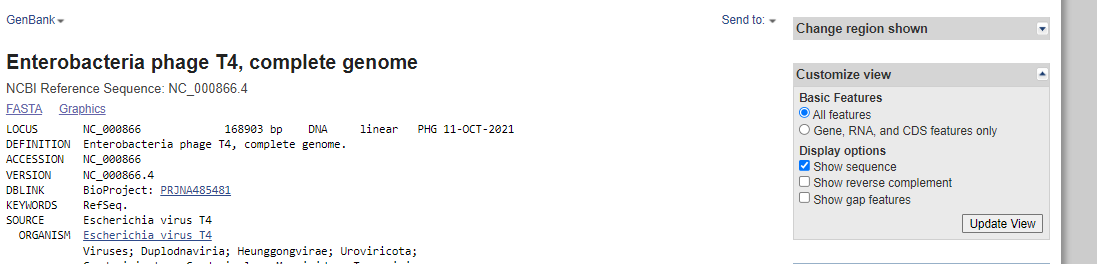
\includegraphics{GenBank.png} At this
point, we can click the ``send to'' button and download the file as a
genebank file (.gb) 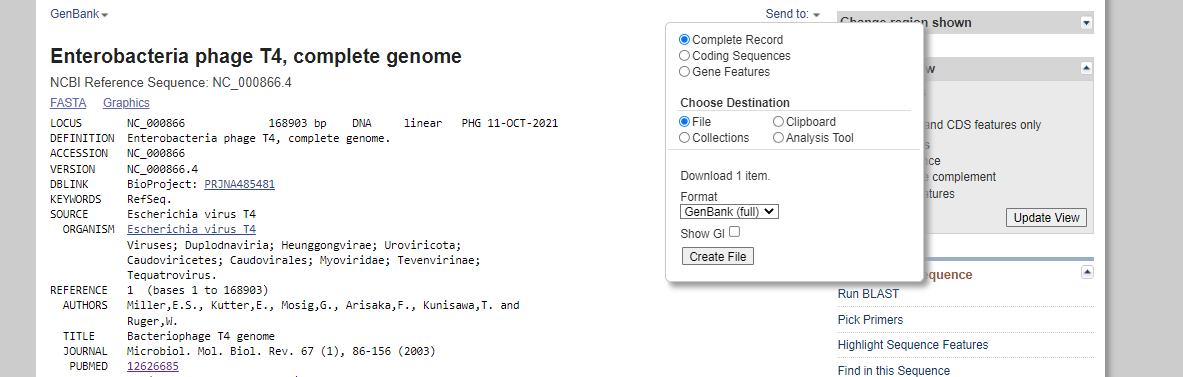
\includegraphics{GenBankDownload.png} Using scp, we
can trasfer the file over to our cluster:

After transferring over the file, we need to check to make sure it
contains the sequence as well as the features. This can be done by
opening the file, and scrolling until you see a header called
``Origin''. Under this should be a sequence with nucleotides.

\begin{Shaded}
\begin{Highlighting}[]
\CommentTok{#cat sequence.gb}

\CommentTok{#We are able to see the nucleotide seqeunce here!}
\end{Highlighting}
\end{Shaded}

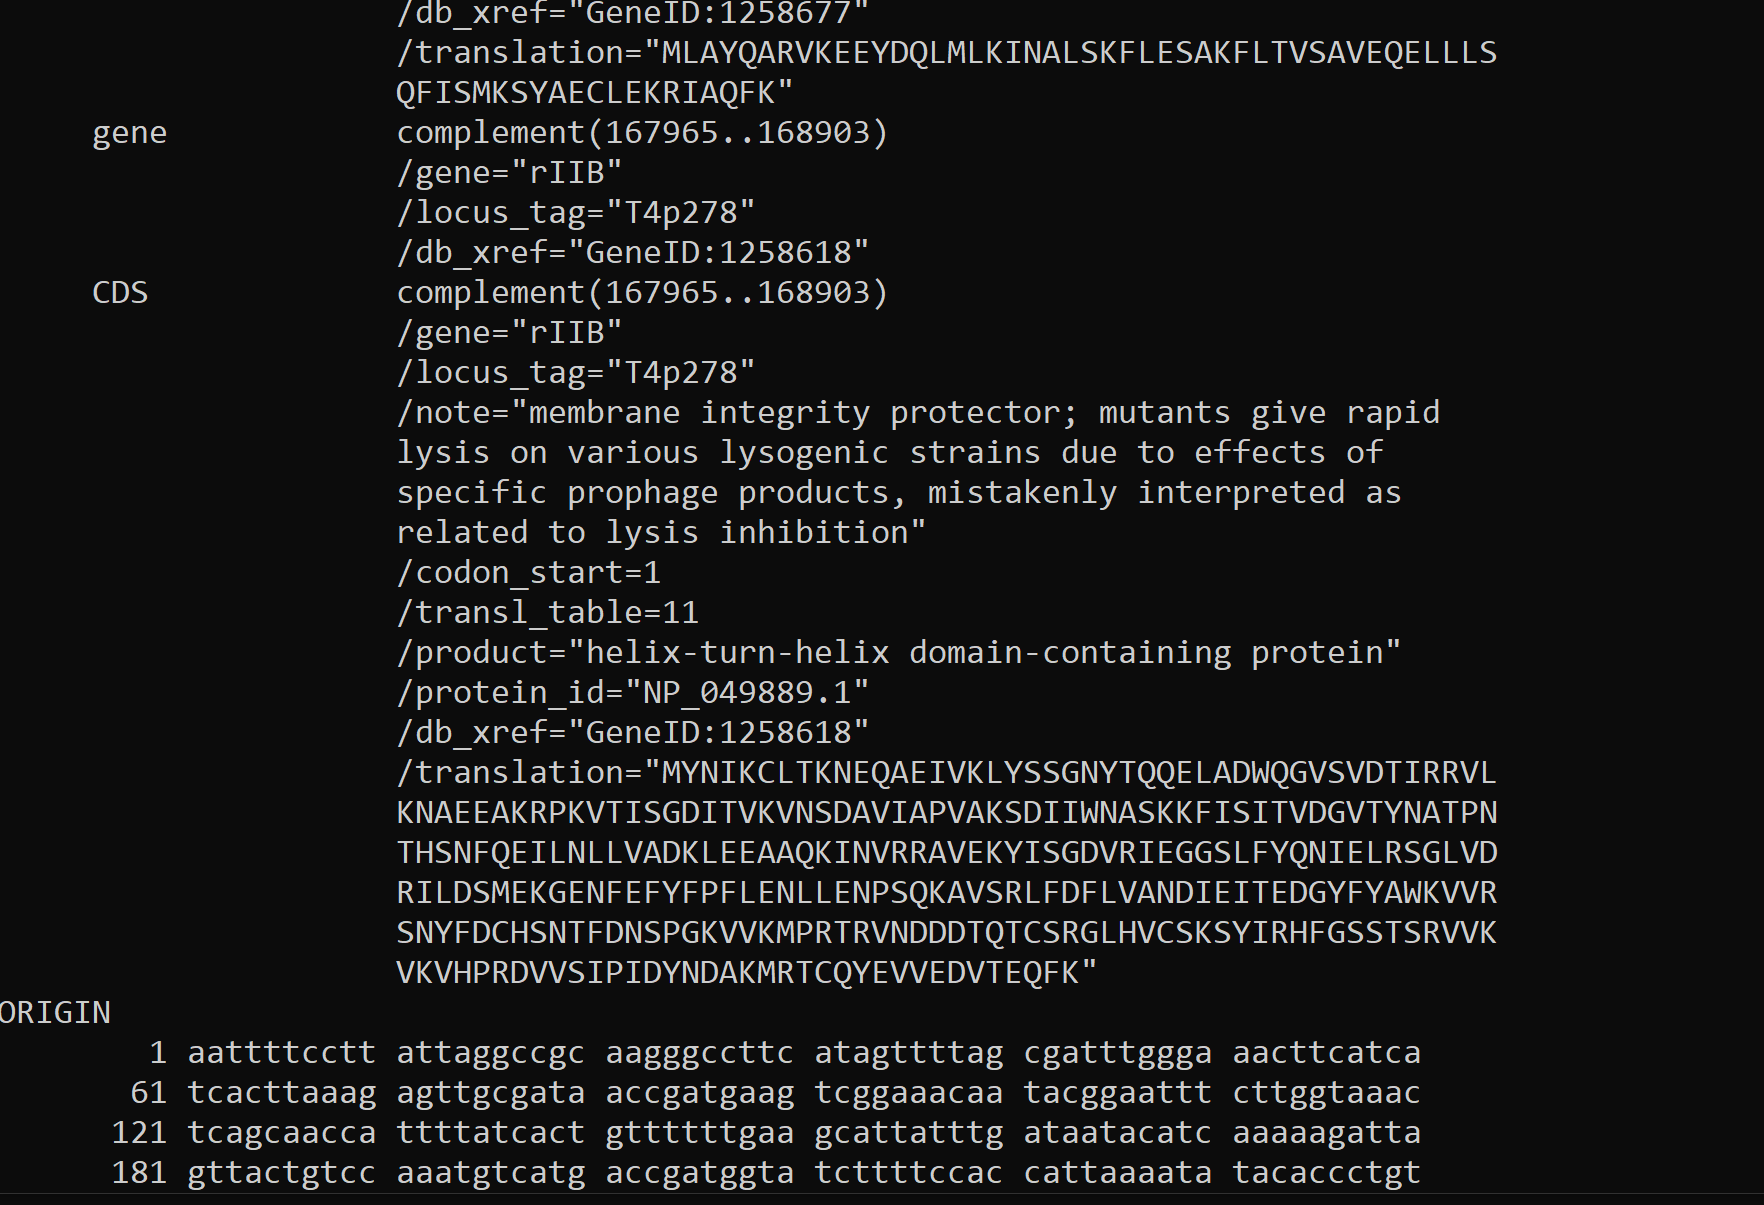
\includegraphics{view_genebank_file.png} We have sucessfully downloaded
the reference genome!

\#Mutation calling pipeline for a single sample: We will now overview
the data analysis pipeline for a single sample (SRR10323947). This
consists of 1) downloading the fastq files from SRA 2) Running fastqc on
the fastq files 3) Using trimmomatic to clean up are fastq files and
remove the illumina adapters. 4) Running fastqc again on the trimmed
samples to confirm trimmmatic was sucessful 5) Running breseq to find
mutations relative to the T4 bacteriophage reference genome.

After this section, we will develop a series of pipelines that does all
of this together. \#\# Step 1: Downloading the fastq file from SRA:

The first step is to download the sequences for each of the 15 samples
from SRA.

\begin{Shaded}
\begin{Highlighting}[]
\CommentTok{#using conda to install the sra tools package}
\CommentTok{#conda install -c bioconda sra-tools}

\CommentTok{#It's important to add the split files command to get both forwards and reverse reads. }
\CommentTok{# fastq-dump SRR10323947 --split-files }
\end{Highlighting}
\end{Shaded}

\#Step 2: Quality control- Running fastqc on the the fastq file:

We can use fastQC to check the quality of our files. This checks the
quality scores of our sequences, and tells us if there is unexpected
coverage, adapter content or unknown nucleotides. This needs to be run
on both the forwards and reverse reads.

\begin{Shaded}
\begin{Highlighting}[]
\CommentTok{#fastqc SRR10323947_1.fastq}
\end{Highlighting}
\end{Shaded}

The read quality drops off significantly near the ends of reads. This
means we will have to use trimmomatic to remove some of the poor quality
bases near the end of every read. This allows downstream analysis with
breseq to only work with high quality data.
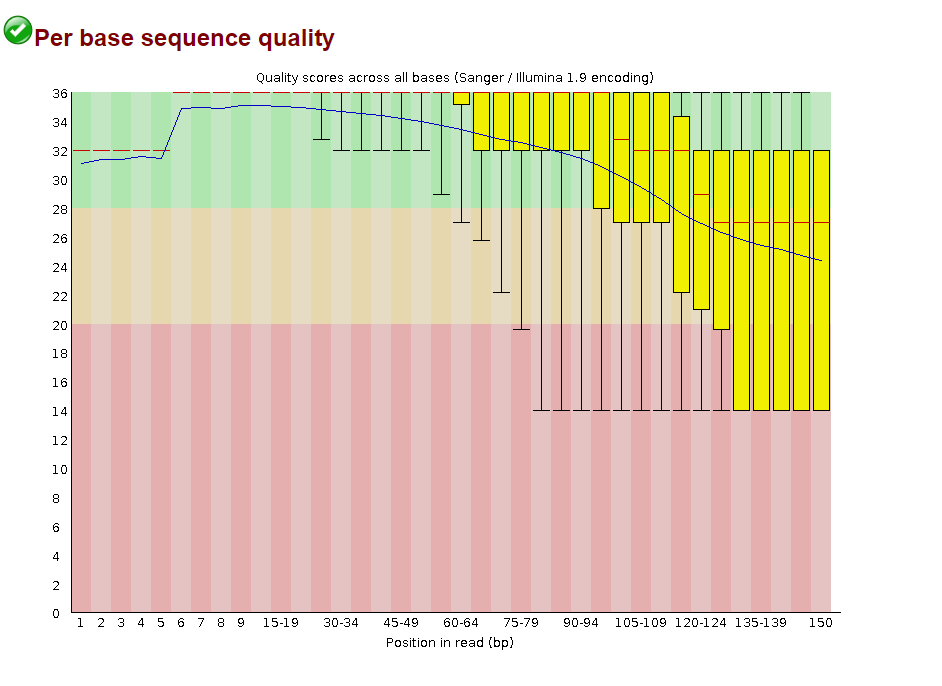
\includegraphics{fastqc_example.png}

\#\#Step 3: Quality control- Using trimmomatic to filter the fastq file
and remove illumina adapters. Next we can use trimmomatic to trim off
the adapter sequences and poor reads near the end. The paper mentions:
``Demultiplexed reads were trimmed for Nextera adapter sequences using
Trimmomatic with default settings''. We also have to trim off the
illumina adapters from our reads, as shows in the photo below
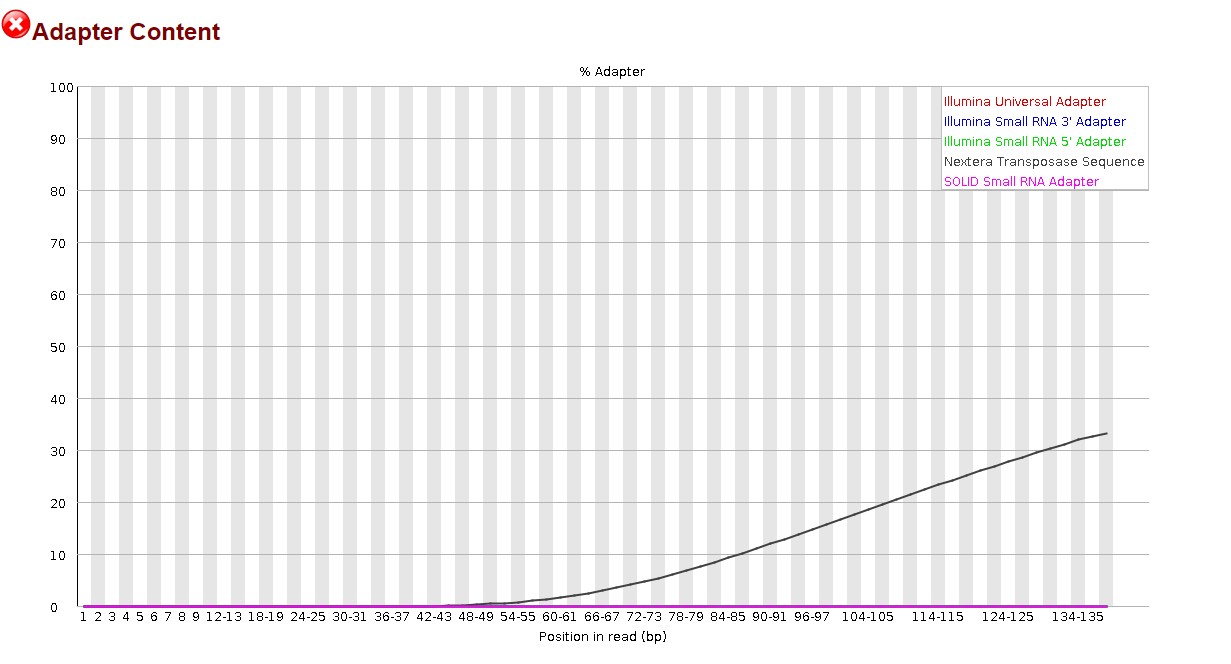
\includegraphics{fastqc_adapters_to_trim.png}

\begin{Shaded}
\begin{Highlighting}[]
\CommentTok{#conda install -c bioconda trimmomatic}

\CommentTok{#First we have to make sure the fastqc files we have are in the zipped format- this makes it faster for trimmomatic. }
\CommentTok{#gzip *.fastq}

\CommentTok{#Next we need to copy the illumina adapters for nextera paired-end sequencing into our working directory. These are downloaded with trimmomatic. }
\CommentTok{#(bmeg400e_env) elyall_bmeg22@orca01:~/anaconda3/pkgs/trimmomatic-0.39-hdfd78af_2/share/trimmomatic/adapters$ cp NexteraPE-PE.fa /home/elyall_bmeg22/final_project/}

\CommentTok{#Now we can run the trimmomatic commands to remove the illumina adapters. The other parameters (sliding window, minlen, 2:40:15) are default parameters taken off the trimmomatic documentation, as the study authors did not say what parameters they used. }

\CommentTok{#trimmomatic PE SRR10323947_1.fastq.gz SRR10323947_2.fastq.gz SRR10323947_1.trim.fastq.gz SRR10323947_1un.trim.fastq.gz SRR10323947_2.trim.fastq.gz SRR10323947_2un.trim.fastq.gz SLIDINGWINDOW:4:20 MINLEN:25 ILLUMINACLIP:NexteraPE-PE.fa:2:40:15}

\CommentTok{#Below is the output of the trimmomatic command: }

\CommentTok{#TrimmomaticPE: Started with arguments:}
\CommentTok{# SRR10323947_1.fastq.gz SRR10323947_2.fastq.gz SRR10323947_1.trim.fastq.gz SRR10323947_1un.trim.fastq.gz SRR10323947_2.trim.fastq.gz #SRR10323947_2un.trim.fastq.gz SLIDINGWINDOW:4:20 MINLEN:25 ILLUMINACLIP:NexteraPE-PE.fa:2:40:15}
\CommentTok{#Using PrefixPair: 'AGATGTGTATAAGAGACAG' and 'AGATGTGTATAAGAGACAG'}
\CommentTok{#Using Long Clipping Sequence: 'GTCTCGTGGGCTCGGAGATGTGTATAAGAGACAG'}
\CommentTok{#Using Long Clipping Sequence: 'TCGTCGGCAGCGTCAGATGTGTATAAGAGACAG'}
\CommentTok{#Using Long Clipping Sequence: 'CTGTCTCTTATACACATCTCCGAGCCCACGAGAC'}
\CommentTok{#Using Long Clipping Sequence: 'CTGTCTCTTATACACATCTGACGCTGCCGACGA'}
\CommentTok{#ILLUMINACLIP: Using 1 prefix pairs, 4 forward/reverse sequences, 0 forward only sequences, 0 reverse only sequences}
\CommentTok{#Quality encoding detected as phred33}
\CommentTok{#Input Read Pairs: 1086157 Both Surviving: 670281 (61.71%) Forward Only Surviving: 393675 (36.24%) Reverse Only Surviving: 13161 (1.21%) #Dropped: 9040 (0.83%)}
\CommentTok{#TrimmomaticPE: Completed successfully}
\end{Highlighting}
\end{Shaded}

\hypertarget{step-4-quality-control--running-an-additional-fastqc-to-confirm-the-adapter-sequences-are-removed}{%
\subsection{Step 4: Quality control- running an additional fastqc to
confirm the adapter sequences are
removed:}\label{step-4-quality-control--running-an-additional-fastqc-to-confirm-the-adapter-sequences-are-removed}}

We now need to run fastq again on our trimmed sample to confirmed if the
adapter contents are actually removed.

\begin{Shaded}
\begin{Highlighting}[]
\CommentTok{#fastqc SRR10323947_1.trim.fastq.gz}
\end{Highlighting}
\end{Shaded}

You can see the the nextera adapter content is now removed. Since the
authors did not make any additional adjustments, neither will we.
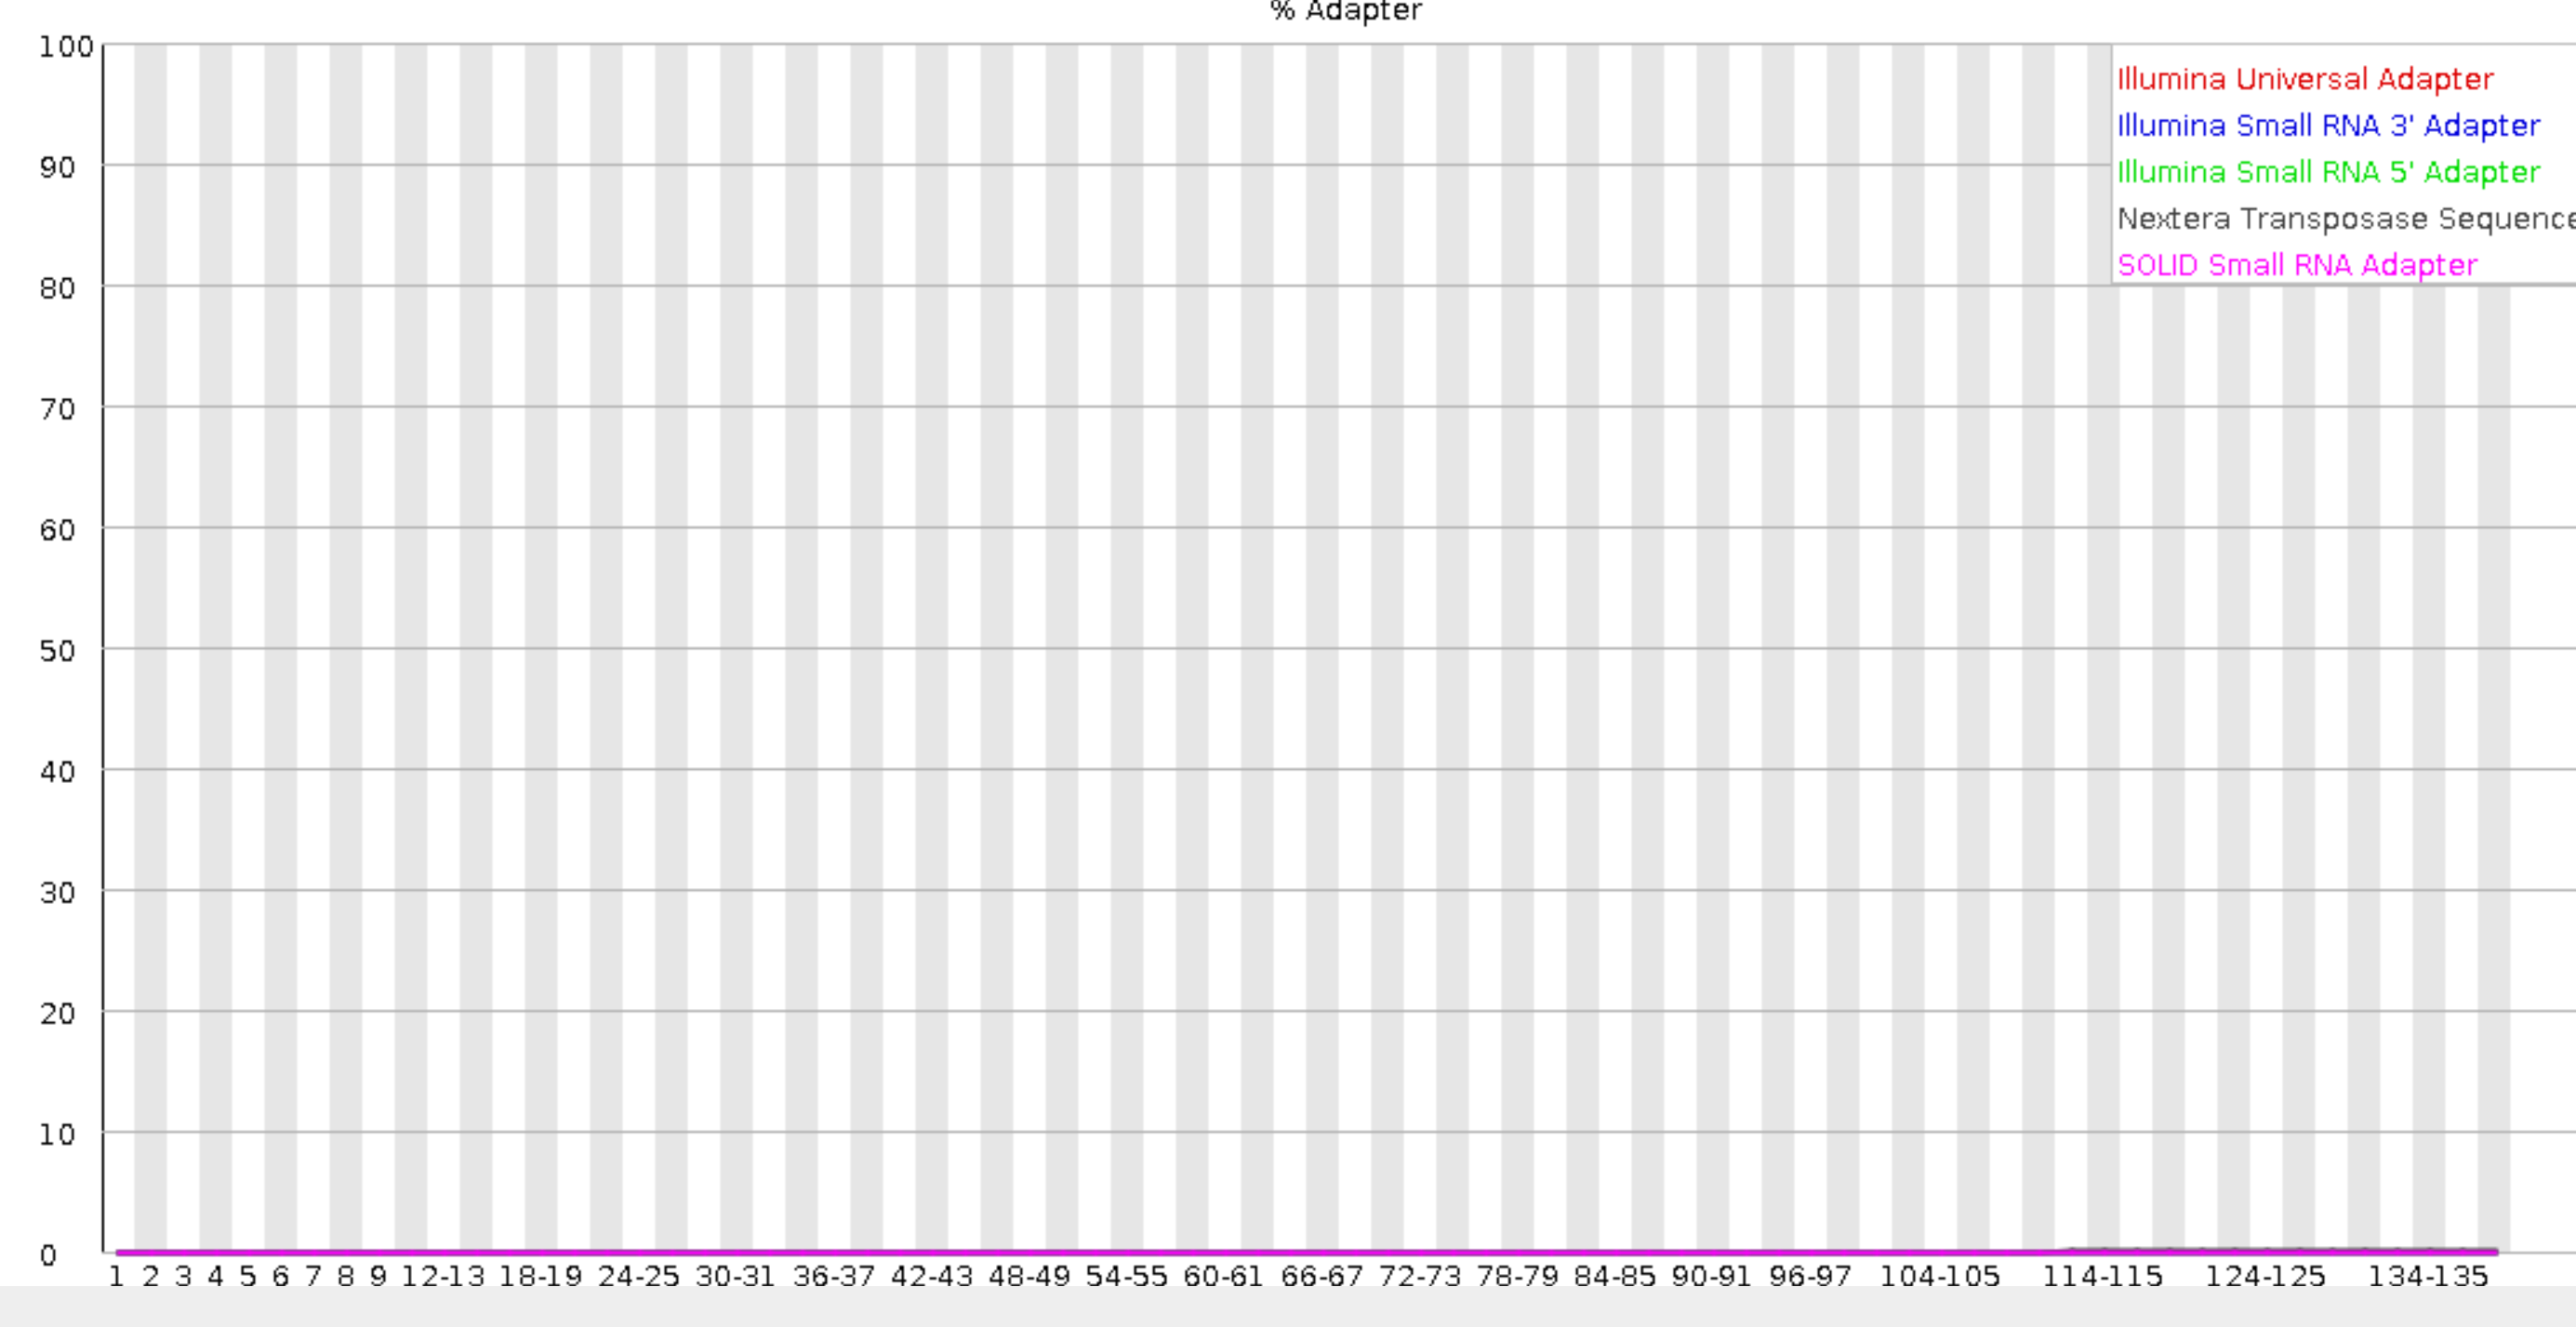
\includegraphics{cleaned_adapters.png} \#\# Step 5: Running breseq to
call mutations on our sample The next step is to download and run
breseq. breseq is a pipeline that is best for calling mutations on small
microbial genomes. It starts by aligning the reads to a reference
sequence, and then looks for consistent mismatches. Breseq can be run in
``population mode'' with the -p flag. This is used when a heterogeneous
population is sequences, and one wants to find all of the possible
mutations against a reference sequence. If greater than 5\% of the reads
at a given position mismatch, breseq reports a mutation at this
position. breseq will report all of the mutations, their frequencies and
positions. It also looks at the reading frame and determines if
mutations are synonymous or non-synonymous, and identified deletions,
insertions and SNP's. Using the genome annotation from the reference
sequence, breseq will report what gene the mutation occurs in and the
function of that gene if it's available. These features make breseq and
incredibly useful tool for analyzing mutations in microbial sequences.

\begin{Shaded}
\begin{Highlighting}[]
\CommentTok{#Breseq requires bowtie and samtools to be installed first. }

\CommentTok{#conda -c bioconda install bowtie}
\CommentTok{#conda -c bioconda install samtools}

\CommentTok{#Now installing breseq}
\CommentTok{#conda -c bioconda install breseq}

\CommentTok{#ARunning breseq on a single sample, where seqeunce.gb is our reference T4 bacteriophage sequene. }
\CommentTok{# breseq -p -r sequence.gb -o /home/elyall_bmeg22/final_project/paired/trimmed_files/breseq_run/ SRR10323947_1.trim.fastq.gz SRR10323947_2.trim.fastq.gz}
\end{Highlighting}
\end{Shaded}

Let's look at some of the output files of our breseq data!

Breseq gives us summary information for each sample. This lets us know
that most of our read are mapped. Breseq requires 90\% of a reads length
to map. 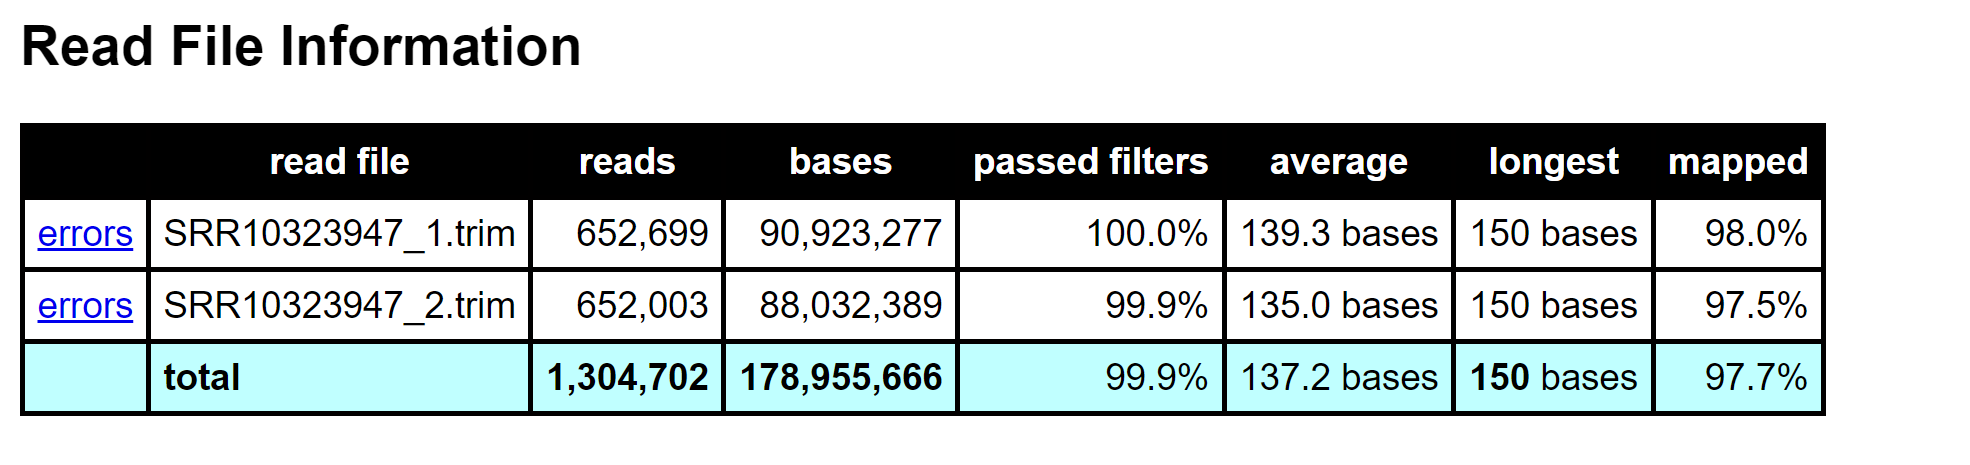
\includegraphics{summary_info.png}

Breseq also give a list of mutation predictions for each sample:

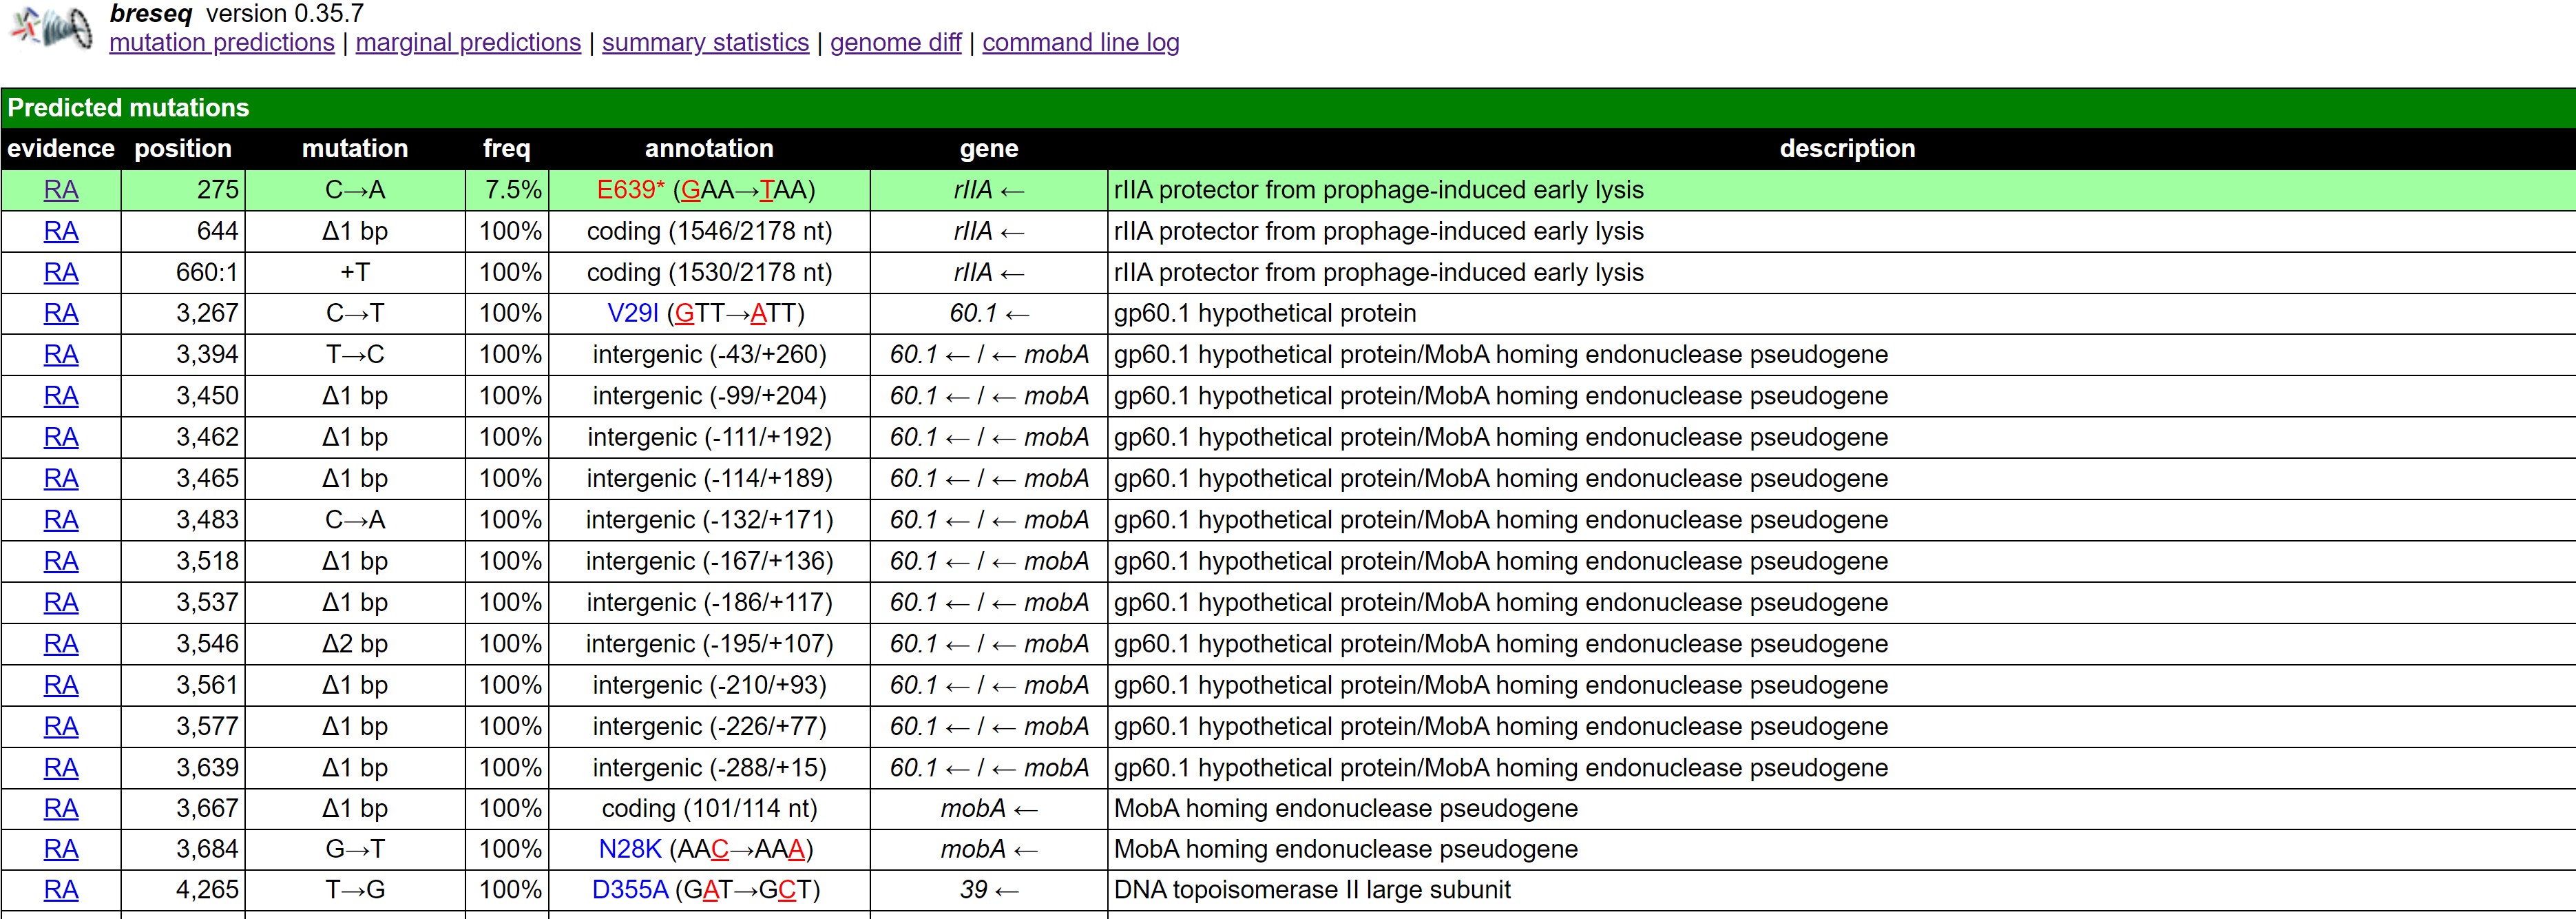
\includegraphics{sample_output.png} If you click on the evidence, it
will show you all of the reads mapping to that position, and highlight
the exptcted mutation. 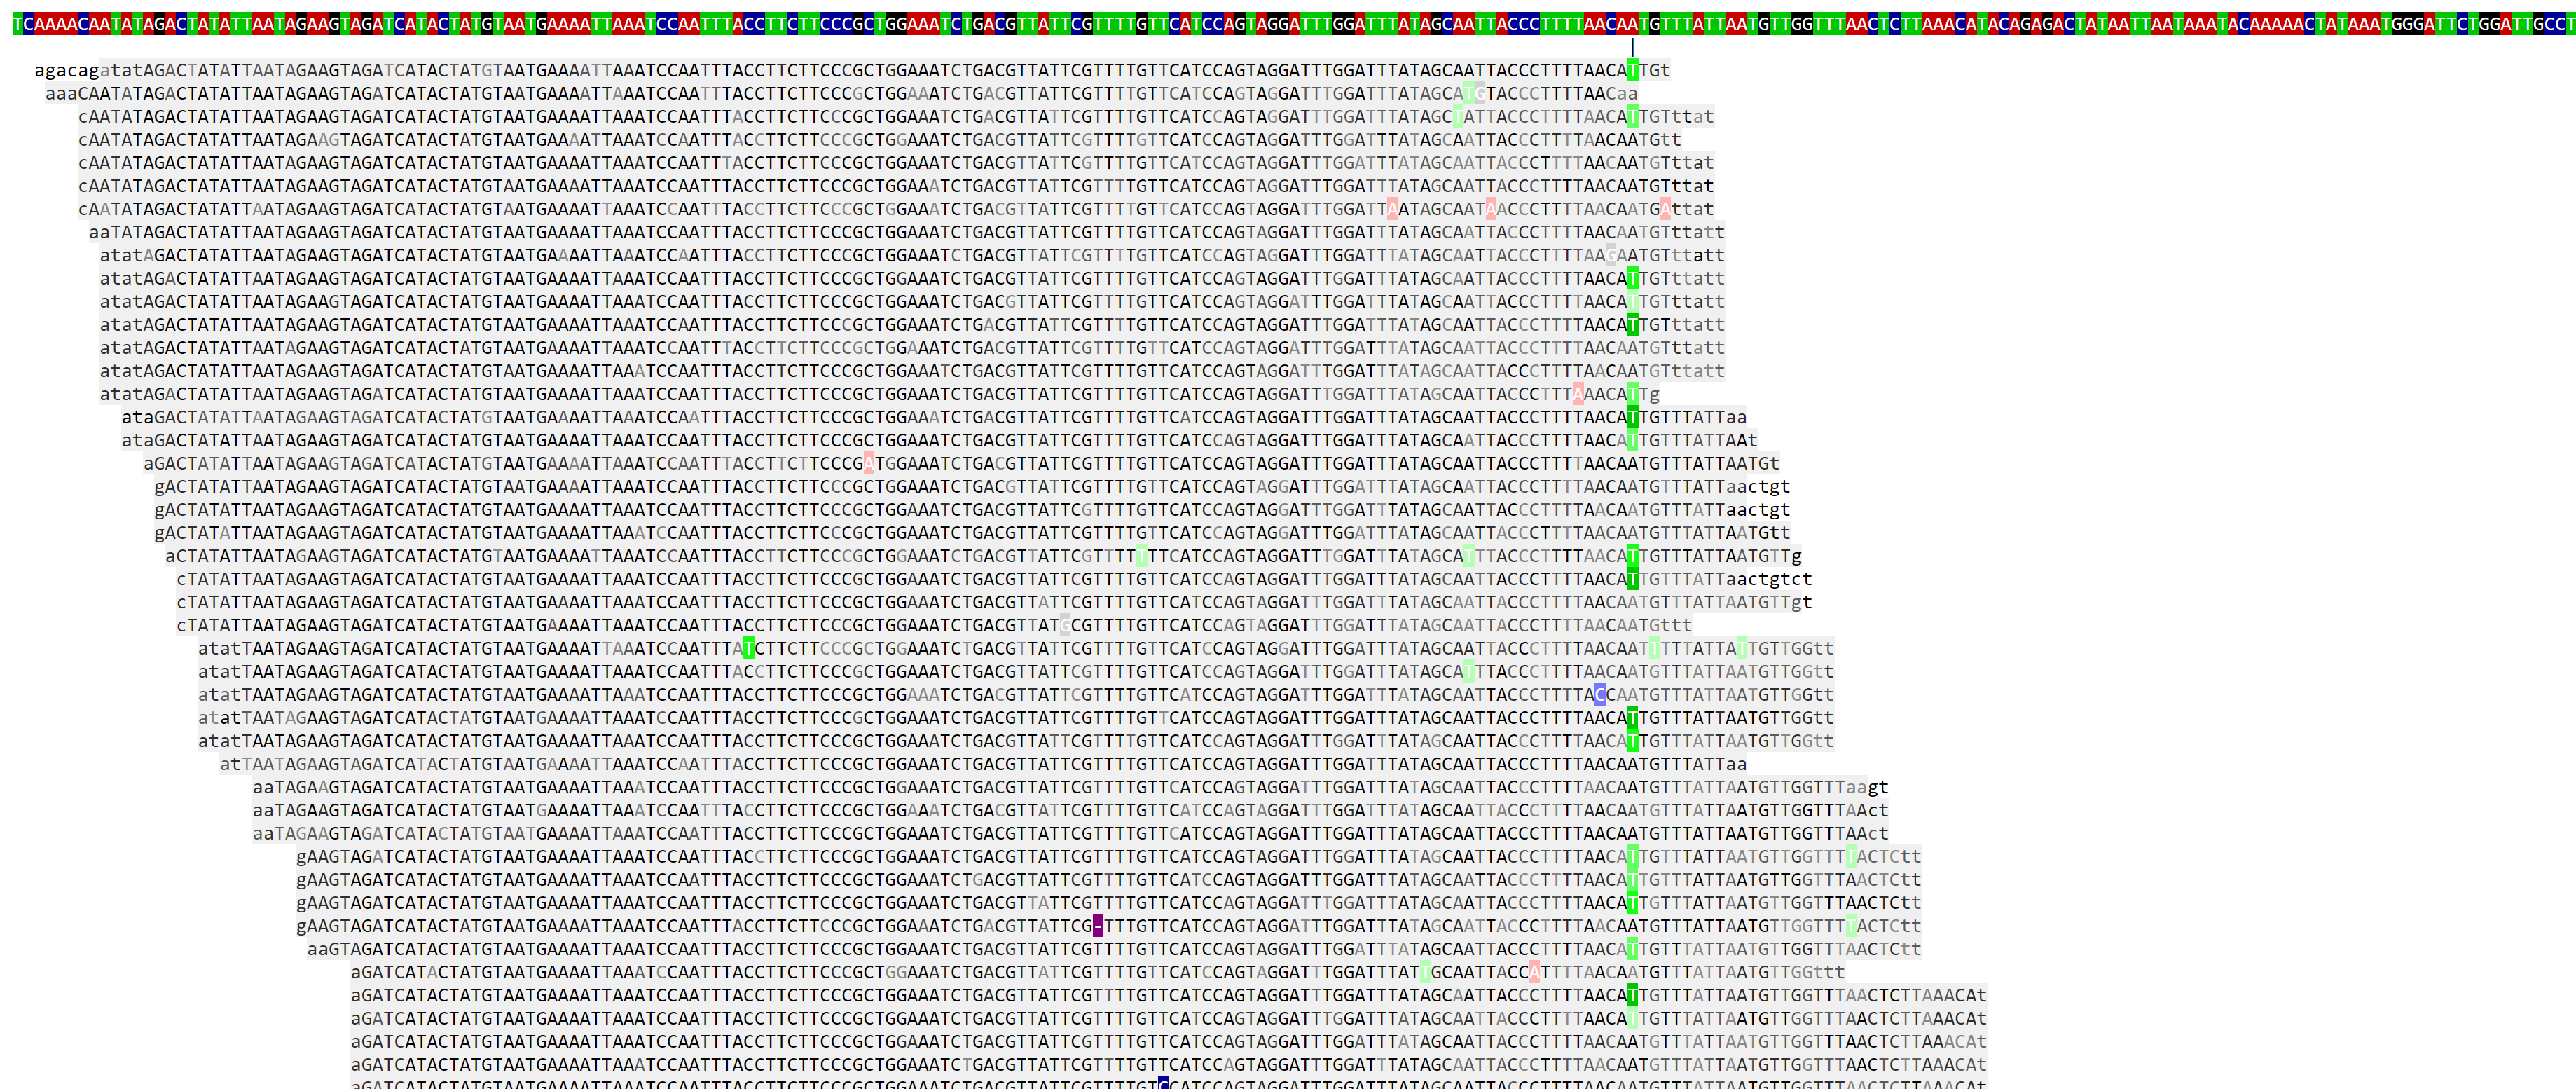
\includegraphics{align_evidence.png}

We can see our coverage is close to 1000 base pairs on average (which is
what the authors aimed to seqeunce at). Breseq highlights
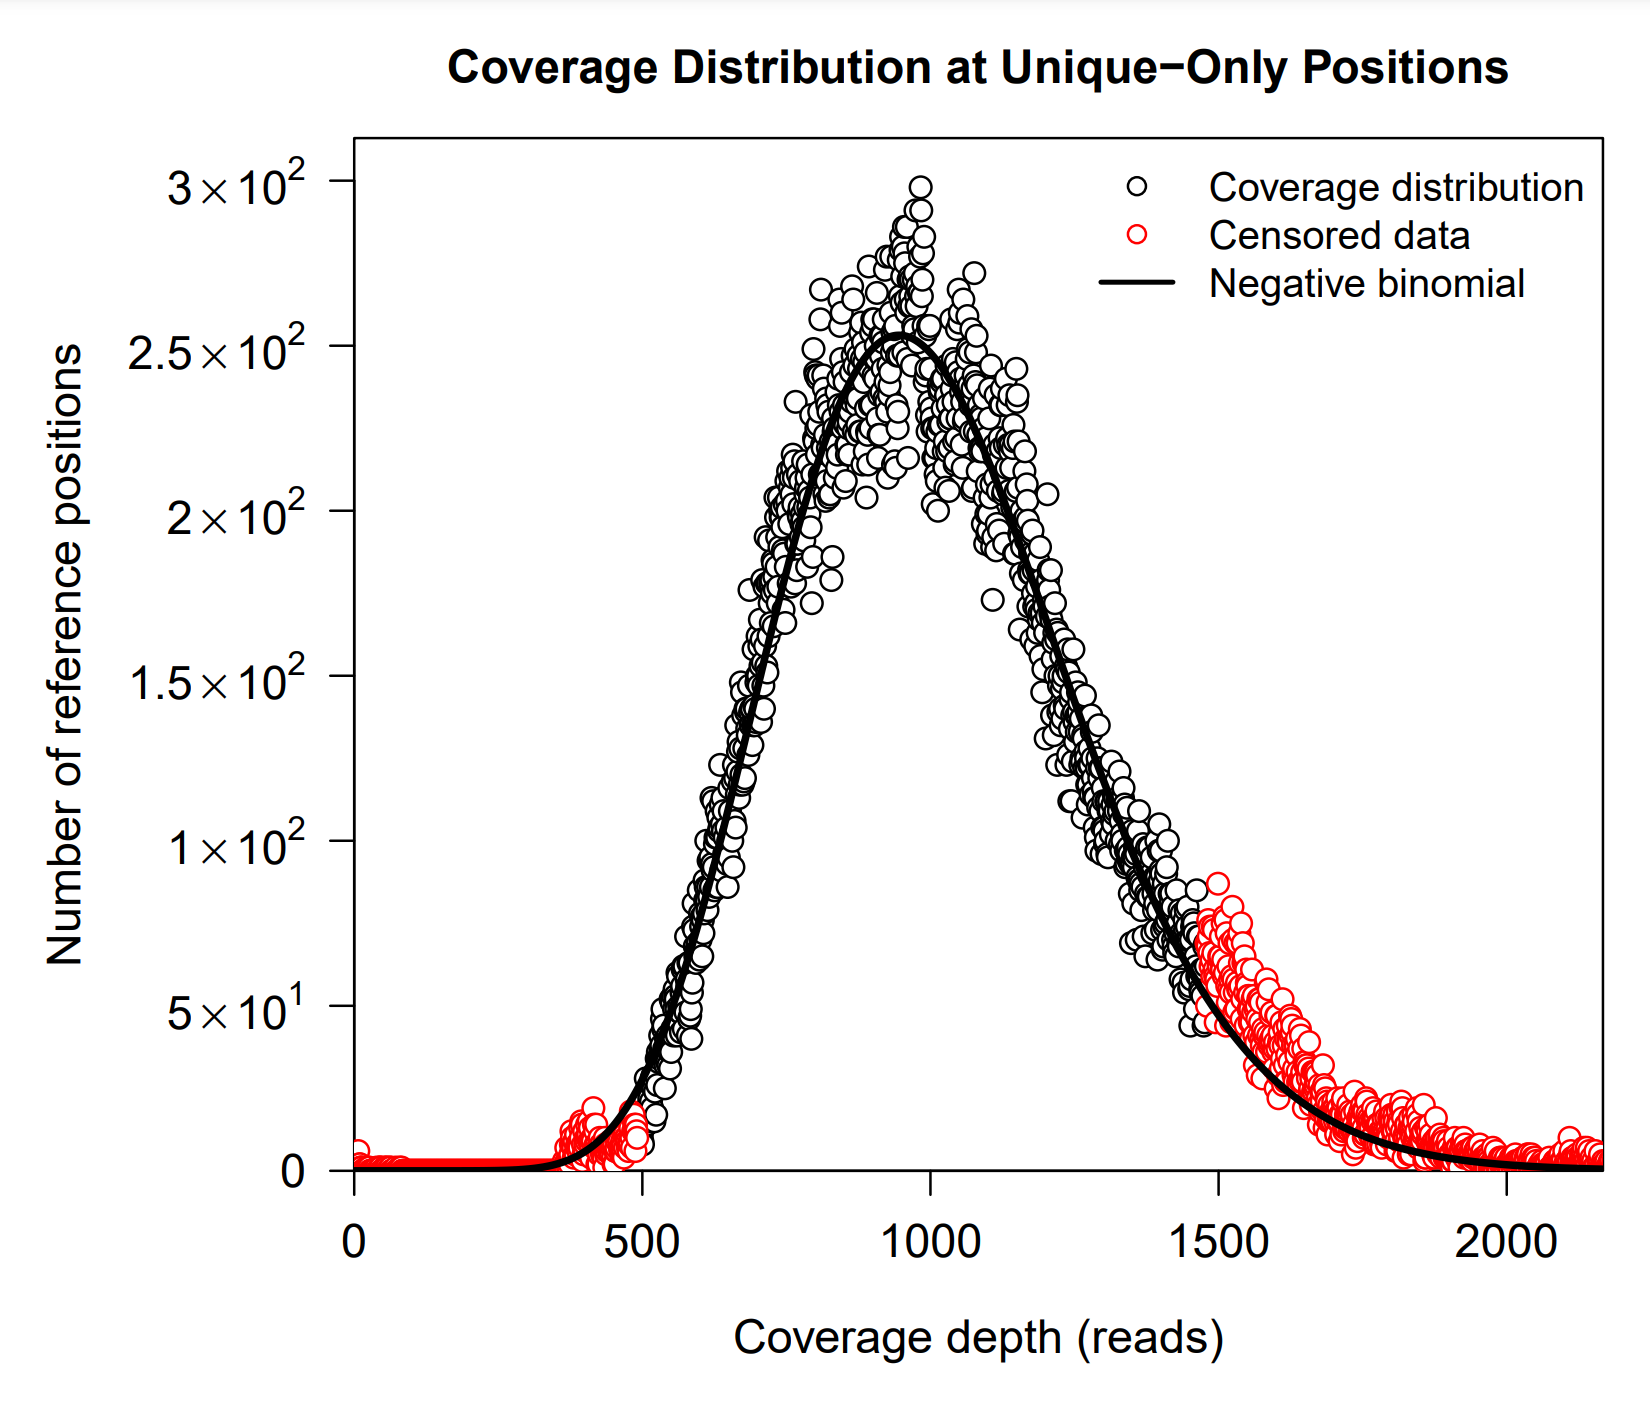
\includegraphics{Coverage_example.png}

\#Creating pipeline to preform analysis on all 15 samples: This section
contains a combination of pipelines that will ultimately run mutation
calling on all 15 of our samples

\#\#Downloading all of the SRA names from NIH: Making a textfile
containing all of the SRA names

\begin{Shaded}
\begin{Highlighting}[]
\CommentTok{#First we have to download the acession list as a txt file form NCBI}
\CommentTok{#https://www.ncbi.nlm.nih.gov/sra?term=SRP226618}

\CommentTok{#creating a .txt file containing all of the SRA #'s for each sample: }
\CommentTok{#nano SRA_seqs.txt }
\CommentTok{#We then copy paste all of the SRA #'s names into this file }
\end{Highlighting}
\end{Shaded}

\#\#Creating a pipeline that downloads fastq files and runs fastQC on
them Now, we are going to generate a pipeline that downloads the fastq
files and runs fastQC on each of these. Normally we would use a job
scheduler to do this, but apparently our server can't do this. So we
will used Dr.~De Boer's script which runs a script for each line in an
input file The script is here:
(\url{https://raw.githubusercontent.com/BMEGGenoInfo/Assignments/main/Assignment_2/runTheseJobsSerially.sh}

\begin{Shaded}
\begin{Highlighting}[]
\CommentTok{#Downloading Carl's script: }

\CommentTok{#wget https://raw.githubusercontent.com/BMEGGenoInfo/Assignments/main/Assignment_2/runTheseJobsSerially.sh}

\CommentTok{#Getting permissions to run it:}
\CommentTok{#chmod +x runTheseJobsSerially.sh}

\CommentTok{#Creating a pipeline called down_trim_pipeline.sh that downloads files from NCBI, runs fastQC and then runs trimmomatic on them. }
\CommentTok{#First we make the name of the pipeline: }
\CommentTok{#nano down_trim_pipeline.sh}

\CommentTok{#Then we get permission on it}
\CommentTok{#chmod +x down_trim_pipeline.sh}

\CommentTok{#Then we run it!}
\CommentTok{#./runTheseJobsSerially.sh ./pipelines/down_trim_pipeline.sh SRA_seqs.txt}

\CommentTok{#The pipeline is shown below:}

\CommentTok{#!/bin/bash}
\CommentTok{#set -e # this makes the whole script exit on any error.}
\CommentTok{#sample=$1}
\CommentTok{#mkdir -p fastq_samples # making a directory to add the fastq files}
\CommentTok{#mkdir -p fastqc_files #making a directory for fastqc_files}
\CommentTok{#mkdir -p downtrim_logfiles}
\CommentTok{##Now, going to run the pipeline: }

\CommentTok{#echo running pipeline for $sample}
\CommentTok{#if [ ! -e downtrim_logfiles/$sample.fastq.done ] }
\CommentTok{#then}
\CommentTok{#        echo Downloading $sample}
\CommentTok{#       #Command download sample:}
\CommentTok{#        fastq-dump $sample --split-files --outdir fastq_samples/}
\CommentTok{#        touch downtrim_logfiles/$sample.fastq.done #add a flag to say fastq downloaded.}
\CommentTok{#else}
\CommentTok{#        echo Already performed fastqc of $sample}
\CommentTok{#        fi}
\CommentTok{#if [ -e downtrim_logfiles/$sample.fastq.done ] #if the fastq is done,do fastqc}
\CommentTok{#then}
\CommentTok{#        echo Running fastqc with $sample}
\CommentTok{#        mkdir fastqc_files/$sample}
\CommentTok{#        fastqc $fastq_samples/\{sample\}_1.fastq --outdir fastqc_files/$sample/}
\CommentTok{#        fastqc $fastq_samples/\{sample\}_2.fastq --outdir fastqc_files/$sample/}
\CommentTok{#        touch downtrim_logfiles/$sample.fastqc.done}
\CommentTok{#else}
\CommentTok{#        echo: FastQC was not made sucessfully.}
\CommentTok{#        fi}
\end{Highlighting}
\end{Shaded}

\#Making a trimmomatic pipeline for all samples We found no additional
concerns beyond the ones mention with our pilot sample in the fastQC.
Before running a trimmomatic pipeline on all of the samples, we have to
gzip the files.

\begin{Shaded}
\begin{Highlighting}[]
\CommentTok{#gzip fastq_samples/*.fastq}

\CommentTok{#Making the name of the trimmomatic pipeline:}

\CommentTok{#nano pipelines/trimmomatic.sh}
\CommentTok{#chmod +x trimmomatic.sh}

\CommentTok{#running the pipeline: }
\CommentTok{#./runTheseJobsSerially.sh ./pipelines/trimmomatic.sh SRA_seqs.txt}
\end{Highlighting}
\end{Shaded}

Below is the code for our trimmomatic pipeline

\begin{Shaded}
\begin{Highlighting}[]
\CommentTok{#!/bin/bash}
\CommentTok{#set -e # this makes the whole script exit on any error.}
\CommentTok{#sample=$1}
\CommentTok{#mkdir -p trimmomatic_files}
\CommentTok{#if [ ! -e downtrim_logfiles/$sample.trim.done ]}
\CommentTok{#then}
\CommentTok{#        mkdir trimmomatic_files/$sample}
\CommentTok{#        trimmomatic PE $fastq_samples/$\{sample\}_1.fastq.gz fastq_samples/$\{sample\}_2.fastq.gz trimmomatic_files/$sample/$\{sample\}_1.trim.fastq.gz trimmomatic_files/$sample/$\{sample\}_1un.trim.fastq.gz trimmomatic_files/$sample/$\{sample\}_2.trim.fastq.gz trimmomatic_files/$sample/$\{sample\}_2un.trim.fastq.gz SLIDINGWINDOW:4:15 MINLEN:25 LEADING:3 TRAILING:3 ILLUMINACLIP:NexteraPE-PE.fa:2:40:15}

\CommentTok{#        touch downtrim_logfiles/$sample.trimmed.done}
\CommentTok{#else}
\CommentTok{#        echo:trimmomatic failed}
\CommentTok{#        fi}
\end{Highlighting}
\end{Shaded}

\#\#Making a pipeline to run breseq This pipeline could have been
attached to the trimmomatic pipeline, but we prefered to run fastQC on
some of the trimmed samples to ensure the trimming is successful. breseq
mutation calling for each sample (1000x coverage, 167k bp) takes 40
minutes.

\begin{Shaded}
\begin{Highlighting}[]
\CommentTok{#Now we make a pipeline to run breseq:}
\CommentTok{# nano pipelines/breseq_pipe.sh}
\CommentTok{# chmod +x breseq_pipe.sh}
\CommentTok{# #Anddd running the pipeline}
\CommentTok{# ./runTheseJobsSerially.sh ./pipelines/breseq_pipe.sh SRA_seqs.txt}
\CommentTok{# }
\CommentTok{# #The pipeline starts below: }
\CommentTok{# }
\CommentTok{# #!/bin/bash}
\CommentTok{# set -e # this makes the whole script exit on any error.}
\CommentTok{# sample=$1}
\CommentTok{# mkdir -p breseq_files}
\CommentTok{# if [ -e downtrim_logfiles/$sample.trimmed.done ]}
\CommentTok{# then}
\CommentTok{#         #Going to run breseq on it}
\CommentTok{#         mkdir -p breseq_files/$sample}
\CommentTok{#         #Running the breseq command:}
\CommentTok{#         # breseq -p -r sequence.gb -o /home/elyall_bmeg22/final_project/breseq_files/$sample/ trimmomatic_files/$sample/$\{sample\}_1.trim.fastq.gz trimmomatic_files/$sample/$\{sample\}_2.trim.fastq.gz}
\CommentTok{#         touch downtrim_logfiles/$sample.breseq.done}
\CommentTok{# else}
\CommentTok{#         echo:breseq failed}
\CommentTok{#         fi}
\end{Highlighting}
\end{Shaded}

\#breseq mutation calling has finished! Typically at this point we would
run a single line of breseq code that would filter all the mutations we
found against the ancestral sequence.

This line would be: gdtools APPLY --f GENBANK --o updated.gbk --r
reference.gbk ancesntral\_input\_sample.gd This takes makes a new
annotated genome (gbk file) contianing all the mutations that are found
in the reference sequence. Future samples would be compared against this
updated gbk file using the gdtools ANNOTATE or COMPARE functions.

However, the author's didn't actually share the data for the ancestral
sample, which is supposed to be compared against the experimental
sample, and have common mutations filtered out. We emailed the author
for these files but nothing came. This is a bit of an issue for us-
keeping all of these mutations in, most of which are from the ancestor,
makes it difficult compare data against the paper, and focus on the
mutations which are important. As a proxy for filtering against the
ancestral sequence, we are going to filter against the final list of
mutations the authors have provided in their supplementary table.

We discussed these changes with Carl and he said we would not lose
difficultly score points here. In our conclusion, we will compare our
results with those of the paper.

Another piece of information we will need is which E.Coli population
each T4 sample evolved on (E.coli C, E.coli K12, or mixed.) This detail
can be found by looking at the sample descriptions on the NCBI
\url{https://www.ncbi.nlm.nih.gov/sra/?term=PRJNA578899} The SRA \#
number is matched to the experimental name and population below:

SRR 61 = 55D18R1 \# E coli K12 replicate 1 SRR 60 = 55D18R2 \#E coli K12
replicate 2 SRR 59 = CD18R1 \#E coli C replicate 1 SRR 58 = CD18R2 \#E
coli C replicate 2 SRR 57 = CD18R3 \#E coli C replicate 3 SRR 56 =
CD18R4 \#E coli C replicate 4 SRR 55 = CD18R5 \#E coli C replicate 5 SRR
54 = 55D18R3 \# E coli K12 replicate 3 SRR 53 = 55D18R4 \# \# E coli K12
replicate 4 SRR 52 = 55D18R5 \# E coli K12 replicate 5 SRR 51 = 55CD18R1
\# alternating e.coli C and K12 replicate 1 SRR 50 = 55CD18R2 \#
alternating e.coli C and K12 replicate 2 SRR 49 =55CD18 R3 \#
alternating e.coli C and K12 replicate 3 SRR 48 = 55CD18R4 \#
alternating e.coli C and K12 replicate 4 SRR 47 = 55CD18R5 \#
alternating e.coli C and K12 replicate 5

\#Annotating our mutations \& filtering against the supplementary table:
To get more detail on our mutations, we can used the ANNOTATE function
from breseq's gdtools. The ANNOTATE tool acts on .gd files. .gd files
are tab-delineated files describing differences between a reference
genome and the tested samples. Currently, our .gd files only contain
detail on what gene was mutated, the base piar change and the positions.
We need more detail for our analysis.\\
The ANNOTATE tool creates an annotated file that adds detail to each
mutation found, including the type (e.g SNP), and whether is synonymous
or non-synonymous. The ANNOTATE function used the reading frame from the
reference equence and determines if the amino acid changes based on
nucleotide changes. We can save this data in a tsv file, where each line
contains a mutation from a sample.

\begin{Shaded}
\begin{Highlighting}[]
\CommentTok{#gdtools ANNOTATE -o annotated_all.tsv -f TSV -r reference_seq.gb 47_output.gd 48_output.gd 49_output.gd 50_output.gd 51_output.gd 52_output.gd 53_output.gd 54_output.gd 55_output.gd 56_output.gd 57_output.gd 58_output.gd 59_output.gd 60_output.gd 61_output.gd}

\CommentTok{#Uploading annotated mutations from a tsv file:: }
\NormalTok{all_ann <-}\StringTok{ }\KeywordTok{as.data.frame}\NormalTok{(}\KeywordTok{read.table}\NormalTok{ (}\DataTypeTok{file =} \StringTok{'annotated_all.tsv'}\NormalTok{, }\DataTypeTok{sep =} \StringTok{'}\CharTok{\textbackslash{}t}\StringTok{'}\NormalTok{, }\DataTypeTok{header =} \OtherTok{TRUE}\NormalTok{))}

\CommentTok{#loading up the supplementary table: }
\KeywordTok{library}\NormalTok{(openxlsx)}
\end{Highlighting}
\end{Shaded}

\begin{verbatim}
## Warning: package 'openxlsx' was built under R version 4.1.3
\end{verbatim}

\begin{Shaded}
\begin{Highlighting}[]
\NormalTok{mutation_xl <-}\StringTok{ }\KeywordTok{read.xlsx}\NormalTok{(}\StringTok{"Supplementary table 2a & 2b.xlsx"}\NormalTok{,}\DataTypeTok{sheet =} \DecValTok{1}\NormalTok{)}
\NormalTok{mutation_df <-}\StringTok{ }\KeywordTok{as.data.frame}\NormalTok{(mutation_xl)}

\CommentTok{#Filtering out the mutation in all_ann that are not in the supplementary files. This is our stand-in for not having the ancestral sequence. }
\CommentTok{#This filtering is done by postion- if there'a mutation called by our team that does not share the position of mutations shown in the paper, we deleted it. }
\KeywordTok{library}\NormalTok{(tidyverse)}
\end{Highlighting}
\end{Shaded}

\begin{verbatim}
## Warning: package 'tidyverse' was built under R version 4.1.3
\end{verbatim}

\begin{verbatim}
## -- Attaching packages --------------------------------------- tidyverse 1.3.1 --
\end{verbatim}

\begin{verbatim}
## v ggplot2 3.3.5     v purrr   0.3.4
## v tibble  3.1.6     v dplyr   1.0.8
## v tidyr   1.2.0     v stringr 1.4.0
## v readr   2.1.2     v forcats 0.5.1
\end{verbatim}

\begin{verbatim}
## Warning: package 'ggplot2' was built under R version 4.1.2
\end{verbatim}

\begin{verbatim}
## Warning: package 'tibble' was built under R version 4.1.2
\end{verbatim}

\begin{verbatim}
## Warning: package 'tidyr' was built under R version 4.1.3
\end{verbatim}

\begin{verbatim}
## Warning: package 'readr' was built under R version 4.1.3
\end{verbatim}

\begin{verbatim}
## Warning: package 'purrr' was built under R version 4.1.2
\end{verbatim}

\begin{verbatim}
## Warning: package 'dplyr' was built under R version 4.1.2
\end{verbatim}

\begin{verbatim}
## Warning: package 'stringr' was built under R version 4.1.2
\end{verbatim}

\begin{verbatim}
## Warning: package 'forcats' was built under R version 4.1.3
\end{verbatim}

\begin{verbatim}
## -- Conflicts ------------------------------------------ tidyverse_conflicts() --
## x dplyr::filter() masks stats::filter()
## x dplyr::lag()    masks stats::lag()
\end{verbatim}

\begin{Shaded}
\begin{Highlighting}[]
\NormalTok{filtered_all_ann <-}\StringTok{ }\KeywordTok{filter}\NormalTok{(all_ann, position }\OperatorTok\StringTok{ }\NormalTok{mutation_df}\OperatorTok{$}\NormalTok{position ) }
\KeywordTok{nrow}\NormalTok{(filtered_all_ann)}
\end{Highlighting}
\end{Shaded}

\begin{verbatim}
## [1] 190
\end{verbatim}

In total we have 192 surviving mutations, compared to the 174 reported
in the paper. This means our analysis is largely successful! Many of the
mutations we found were also found in the paper.

This is much better than what we had before filtering, which was 3197
mutations (most of which are probably from the ancestor)

This means many of the mutations were shared between our data and the
paper's data. We may have more mutations because the there could be
mutations that we have (ancestral or otherwise) which share the same
position. As we have no way of distinguishing these, we will leave them
in for our analysis

\#Annotating our mutation list with functional gene categories Now we
are going to further annotate our mutation list with the gene functional
categories. The authors of this paper took functional gene categories
from a paper by Miller et al (the same paper that made the latest
version of the T4 genome. We've downloaded these functional gene
categories into an excel file, added it to the supplementary table and
will use them for annotation. The purpose of annotating genes by
functional category is to make data visualization eaiser. If we only
have the names of specific genes, it's difficult to get a picture of
what the broad themes were during the evolution of these phage. By
annotating our mutations with functional categories, we are eventually
able to present strong evidence that the mutations in structural viron
proteins drive the niche evolution of bacteriophage.

\begin{Shaded}
\begin{Highlighting}[]
\CommentTok{#First we have to upload each functional category and their associated genes. These designations are taken from the a paper by Miller et al, which was used in this study. }
\CommentTok{#The "functional designations" are: Transcription, Translation, Nucleotide_metabolism, DNA_rep, Virion_prots, chaperonins, lysis, host_phage_int    host_alt, homing_endonuclease, predicted_integral_membrane}
\CommentTok{#Any gene that doesn't fit in one of these categories is classified as unknown.}

\KeywordTok{library}\NormalTok{(openxlsx)}
\NormalTok{func_des <-}\StringTok{ }\KeywordTok{read.xlsx}\NormalTok{(}\StringTok{"Supplementary table 2a & 2b.xlsx"}\NormalTok{,}\DataTypeTok{sheet =} \StringTok{'melt_cat_genes'}\NormalTok{)}
\NormalTok{func_des_df <-}\StringTok{ }\KeywordTok{as.data.frame}\NormalTok{(func_des) }\CommentTok{#functional designation dataframe contains functional categories and their genes. }

\CommentTok{#Now, we can annotate all of our mutation with their matching functional designation. }
\CommentTok{#If no functional designation is found, we will label it as unknown}

\CommentTok{#We are going to iterate through each gene from our mutation data, and assign a gene designation to it:}
\NormalTok{all_genes <-}\StringTok{ }\NormalTok{filtered_all_ann}\OperatorTok{$}\NormalTok{gene_name }\CommentTok{#geting a list of all the genes in our annotated mutation calls from each sample}
\NormalTok{all_genes_func <-}\StringTok{ }\KeywordTok{c}\NormalTok{() }\CommentTok{#Creating an empty vector where associated functional categories will be added}
\ControlFlowTok{for}\NormalTok{(gene }\ControlFlowTok{in}\NormalTok{ all_genes)}
\NormalTok{\{}
\NormalTok{        r <-}\StringTok{ }\KeywordTok{which}\NormalTok{(func_des_df}\OperatorTok{$}\NormalTok{gene }\OperatorTok{==}\StringTok{ }\NormalTok{gene) }\CommentTok{#getting a list of rows where the mutated gene is associated iwth a functional category}
        \ControlFlowTok{if}\NormalTok{(}\KeywordTok{length}\NormalTok{(r)}\OperatorTok{==}\DecValTok{0}\NormalTok{)\{ }\CommentTok{#if we can't find a funcional category associated with the gene}
\NormalTok{                all_genes_func <-}\StringTok{ }\KeywordTok{c}\NormalTok{(all_genes_func,}\StringTok{"unknown"}\NormalTok{) }\CommentTok{#Say the gene function is unknown}
\NormalTok{        \}}
        \ControlFlowTok{else}\NormalTok{\{}
\NormalTok{                all_genes_func <-}\StringTok{ }\KeywordTok{c}\NormalTok{(all_genes_func,func_des_df}\OperatorTok{$}\NormalTok{function_cat[r]) }\CommentTok{#otherwise, add the functional category}
\NormalTok{        \}}
\NormalTok{\}}

\CommentTok{#Adding the vector containing all the gene functional designations to our datframe}
\NormalTok{filtered_all_ann}\OperatorTok{$}\NormalTok{gene_function <-}\StringTok{ }\NormalTok{all_genes_func}
\end{Highlighting}
\end{Shaded}

\#Calculating mutations per functional category: Now we can start
looking at mutations as they relate to functional categories. As with
the paper, mutations are dominated by those in the virion protein
category. This makes sense- modifying virion proteins is one of the
easier ways for phage to increase their infection efficiency over a long
period of evolution. Viron proteins (like tail fibers) facilitate entry
into E.coli, which is required for phage replication and survival.

\begin{Shaded}
\begin{Highlighting}[]
\CommentTok{#Finding the number of mutations per functional category:}
\KeywordTok{library}\NormalTok{(tibble)}
\KeywordTok{library}\NormalTok{(ggplot2)}
\NormalTok{mut_per_func <-}\StringTok{ }\NormalTok{filtered_all_ann }\OperatorTok\StringTok{ }\KeywordTok{group_by}\NormalTok{(gene_function) }\OperatorTok\StringTok{ }\KeywordTok{summarise}\NormalTok{(}\DataTypeTok{n=}\KeywordTok{n}\NormalTok{()) }\OperatorTok\StringTok{ }\KeywordTok{arrange}\NormalTok{(}\KeywordTok{desc}\NormalTok{(n))}
\KeywordTok{ggplot}\NormalTok{(mut_per_func, }\KeywordTok{aes}\NormalTok{(}\DataTypeTok{x=}\StringTok{""}\NormalTok{,}\DataTypeTok{y=}\NormalTok{n,}\DataTypeTok{fill =}\NormalTok{ gene_function))}\OperatorTok{+}\StringTok{ }\KeywordTok{geom_bar}\NormalTok{(}\DataTypeTok{width =} \DecValTok{1}\NormalTok{, }\DataTypeTok{stat =} \StringTok{"identity"}\NormalTok{)}\OperatorTok{+}\StringTok{ }\KeywordTok{ylab}\NormalTok{(}\StringTok{"Number of mutations"}\NormalTok{)}\OperatorTok{+}\StringTok{ }\KeywordTok{xlab}\NormalTok{(}\StringTok{"All mutation frequencies"}\NormalTok{)}
\end{Highlighting}
\end{Shaded}

\includegraphics{final_project_markdown_file_files/figure-latex/unnamed-chunk-14-1.pdf}

\begin{Shaded}
\begin{Highlighting}[]
\CommentTok{#Finding the number of higher-frequency mutations (greater than 50%) per functional category:}
\NormalTok{high_freq <-}\StringTok{ }\NormalTok{filtered_all_ann }\OperatorTok\StringTok{ }\KeywordTok{filter}\NormalTok{(frequency }\OperatorTok{>}\StringTok{ }\FloatTok{.5}\NormalTok{)}
\NormalTok{high_f_mut_func <-}\StringTok{ }\NormalTok{high_freq }\OperatorTok\StringTok{ }\KeywordTok{group_by}\NormalTok{(gene_function) }\OperatorTok\StringTok{ }\KeywordTok{summarise}\NormalTok{(}\DataTypeTok{n=}\KeywordTok{n}\NormalTok{()) }\OperatorTok\StringTok{ }\KeywordTok{arrange}\NormalTok{(}\KeywordTok{desc}\NormalTok{(n))}
\KeywordTok{ggplot}\NormalTok{(high_f_mut_func, }\KeywordTok{aes}\NormalTok{(}\DataTypeTok{x=}\StringTok{""}\NormalTok{,}\DataTypeTok{y=}\NormalTok{n,}\DataTypeTok{fill =}\NormalTok{ gene_function))}\OperatorTok{+}\StringTok{ }\KeywordTok{geom_bar}\NormalTok{(}\DataTypeTok{width =} \DecValTok{1}\NormalTok{, }\DataTypeTok{stat =} \StringTok{"identity"}\NormalTok{) }\OperatorTok{+}\StringTok{ }\KeywordTok{ylab}\NormalTok{(}\StringTok{"Number of mutations"}\NormalTok{) }\OperatorTok{+}\StringTok{ }\KeywordTok{xlab}\NormalTok{(}\StringTok{"Mutations greater than 50% frequency"}\NormalTok{)}
\end{Highlighting}
\end{Shaded}

\includegraphics{final_project_markdown_file_files/figure-latex/unnamed-chunk-14-2.pdf}

\#Comparing mutations by type Next we will get a breakdown of what kinds
of mutations occured in our dataset. From the annotated mutation file,
we get information on whether the mutation was an indel, SNP or
substitution. We also get details on the impact of these mutations
(whether they are synonymous, non-synonymous, non-sense or intergenic).
The purpose of this is twofold. First, it acts as a sanity check- most
of the mutations reported should be SNP's, as these are much less likely
to result in a dysfuctional bacteriophage. Second, this breakdown will
give us a grasp on what kind of mutations are in the dataset, aiding
downstream analysis.

\begin{Shaded}
\begin{Highlighting}[]
\KeywordTok{library}\NormalTok{(dplyr)}
\KeywordTok{library}\NormalTok{(ggplot2)}

\CommentTok{#Getting the total number of mutations}
\KeywordTok{nrow}\NormalTok{(filtered_all_ann)}
\end{Highlighting}
\end{Shaded}

\begin{verbatim}
## [1] 190
\end{verbatim}

\begin{Shaded}
\begin{Highlighting}[]
\CommentTok{#There are 190 mutations in total}

\NormalTok{x =}\StringTok{ }\KeywordTok{data.frame}\NormalTok{(}\KeywordTok{table}\NormalTok{(filtered_all_ann}\OperatorTok{$}\NormalTok{type))}
\KeywordTok{names}\NormalTok{(x)[}\KeywordTok{names}\NormalTok{(x) }\OperatorTok{==}\StringTok{ "Var1"}\NormalTok{] <-}\StringTok{ "Mutation_Type"}
\KeywordTok{names}\NormalTok{(x)[}\KeywordTok{names}\NormalTok{(x) }\OperatorTok{==}\StringTok{ "Freq"}\NormalTok{] <-}\StringTok{ "Frequency"}
\NormalTok{p =}\StringTok{ }\KeywordTok{ggplot}\NormalTok{(}\DataTypeTok{data=}\NormalTok{x, }\KeywordTok{aes}\NormalTok{(}\DataTypeTok{x=}\NormalTok{Mutation_Type, }\DataTypeTok{y=}\NormalTok{Frequency, }\DataTypeTok{fill =}\NormalTok{ Mutation_Type)) }\OperatorTok{+}
\StringTok{  }\KeywordTok{geom_bar}\NormalTok{(}\DataTypeTok{stat=}\StringTok{"identity"}\NormalTok{)}\OperatorTok{+}
\StringTok{  }\KeywordTok{geom_text}\NormalTok{(}\KeywordTok{aes}\NormalTok{(}\DataTypeTok{label=}\NormalTok{Frequency), }\DataTypeTok{vjust=}\OperatorTok{-}\FloatTok{0.3}\NormalTok{, }\DataTypeTok{size=}\FloatTok{3.5}\NormalTok{)}\OperatorTok{+}
\StringTok{  }\KeywordTok{theme_minimal}\NormalTok{()}

\NormalTok{p}
\end{Highlighting}
\end{Shaded}

\includegraphics{final_project_markdown_file_files/figure-latex/unnamed-chunk-15-1.pdf}

\begin{Shaded}
\begin{Highlighting}[]
\CommentTok{#Looking at specifically the SNP mutations to find out how many are synonymous, and how many are non-synonymous, and how many are intergenic}
\NormalTok{filtered_all_ann_noNonSNP <-}\StringTok{ }\NormalTok{filtered_all_ann[filtered_all_ann}\OperatorTok{$}\NormalTok{type }\OperatorTok{==}\StringTok{ 'SNP'}\NormalTok{,]}
\NormalTok{y =}\StringTok{ }\KeywordTok{data.frame}\NormalTok{(}\KeywordTok{table}\NormalTok{(filtered_all_ann_noNonSNP}\OperatorTok{$}\NormalTok{snp_type))}
\KeywordTok{names}\NormalTok{(y)[}\KeywordTok{names}\NormalTok{(y) }\OperatorTok{==}\StringTok{ "Var1"}\NormalTok{] <-}\StringTok{ "SNP_Type"}
\KeywordTok{names}\NormalTok{(y)[}\KeywordTok{names}\NormalTok{(y) }\OperatorTok{==}\StringTok{ "Freq"}\NormalTok{] <-}\StringTok{ "Frequency"}
\NormalTok{p =}\StringTok{ }\KeywordTok{ggplot}\NormalTok{(}\DataTypeTok{data=}\NormalTok{y, }\KeywordTok{aes}\NormalTok{(}\DataTypeTok{x=}\NormalTok{SNP_Type, }\DataTypeTok{y=}\NormalTok{Frequency, }\DataTypeTok{fill =}\NormalTok{ SNP_Type)) }\OperatorTok{+}
\StringTok{  }\KeywordTok{geom_bar}\NormalTok{(}\DataTypeTok{stat=}\StringTok{"identity"}\NormalTok{)}\OperatorTok{+}
\StringTok{  }\KeywordTok{geom_text}\NormalTok{(}\KeywordTok{aes}\NormalTok{(}\DataTypeTok{label=}\NormalTok{Frequency), }\DataTypeTok{vjust=}\OperatorTok{-}\FloatTok{0.3}\NormalTok{, }\DataTypeTok{size=}\FloatTok{3.5}\NormalTok{)}\OperatorTok{+}
\StringTok{  }\KeywordTok{theme_minimal}\NormalTok{()}

\NormalTok{p}
\end{Highlighting}
\end{Shaded}

\includegraphics{final_project_markdown_file_files/figure-latex/unnamed-chunk-15-2.pdf}

\#Finding the number of mutations that are fixed and not fixed. Next we
will analyze the number of mutations that are fixed and not fixed. A
fixed mutation will be defined at over 80\% prevelance in the population
- meaning these mutations were either essential, or associated with
other essential mutations that gave the bacterophage a competitiva
advantage while evolved. Non-fixed mtuations will be defined as
mutations with a population frequency from 5-80\%. These mutations
occured, but their consequences are not strong enough to either a)
vanish entirely by being out competed or b) become fully ingrained in
the population (fixed). The pupose of doing this analysis is to see
whether or not selection occured on the evolved populations. If
selection occurs, we should see two things: 1) There should be a portion
of mutations that become fixed in the population 2) The mutations that
do become fixed should be mostly non-synonymous, resulting in an amino
acid change. It would make little sense if the fixed mutations were all
silent synonymous mutations, because these should not exert evolutionary
pressure. As you can see in the graphs below, the majority of SNP
mutations were non-synonymous, particulary in the fixed mutation
category. This indicates selection occurred during the experiment. These
results are in line with the reported results from the paper.

\begin{Shaded}
\begin{Highlighting}[]
\CommentTok{# trying to generate some graphs by fixed/non-fixed status, as in the paper}
\KeywordTok{library}\NormalTok{(ggplot2)}
\KeywordTok{library}\NormalTok{(dplyr)}
\CommentTok{# add bacterial population labels}
\NormalTok{b_pop_dict <-}\StringTok{ }\KeywordTok{c}\NormalTok{(}\StringTok{"47_output"}\NormalTok{ =}\StringTok{ 'Alternating C & K12'}\NormalTok{, }\StringTok{"48_output"}\NormalTok{ =}\StringTok{ 'Alternating C & K12'}\NormalTok{, }\StringTok{"49_output"}\NormalTok{ =}\StringTok{ 'Alternating C & K12'}\NormalTok{, }\StringTok{"50_output"}\NormalTok{ =}\StringTok{'Alternating C & K12'}\NormalTok{, }\StringTok{"51_output"}\NormalTok{ =}\StringTok{ 'Alternating C & K12'}\NormalTok{, }\StringTok{"52_output"}\NormalTok{=}\StringTok{ 'E.coli K12'}\NormalTok{, }\StringTok{"53_output"}\NormalTok{ =}\StringTok{ 'E.coli K12'}\NormalTok{, }\StringTok{"54_output"}\NormalTok{ =}\StringTok{ 'E.coli K12'}\NormalTok{, }\StringTok{"55_output"}\NormalTok{ =}\StringTok{'E.coli C'}\NormalTok{ , }\StringTok{"56_output"}\NormalTok{ =}\StringTok{'E.coli C'}\NormalTok{ , }\StringTok{"57_output"}\NormalTok{=}\StringTok{ 'E.coli C'}\NormalTok{, }\StringTok{"58_output"}\NormalTok{=}\StringTok{ 'E.coli C'}\NormalTok{ , }\StringTok{"59_output"}\NormalTok{=}\StringTok{ 'E.coli C'}\NormalTok{ , }\StringTok{"60_output"}\NormalTok{ =}\StringTok{ 'E.coli K12'}\NormalTok{, }\StringTok{"61_output"}\NormalTok{ =}\StringTok{'E.coli K12'}\NormalTok{ )}
\NormalTok{population_y_axis_vals <-}\StringTok{ }\KeywordTok{c}\NormalTok{()}
\NormalTok{output_names <-}\StringTok{ }\NormalTok{filtered_all_ann}\OperatorTok{$}\NormalTok{title}
\ControlFlowTok{for}\NormalTok{(output_name }\ControlFlowTok{in}\NormalTok{ output_names)\{}
\NormalTok{  y_val <-}\StringTok{ }\NormalTok{b_pop_dict[output_name]}
\NormalTok{  population_y_axis_vals <-}\StringTok{ }\KeywordTok{c}\NormalTok{(population_y_axis_vals,y_val)}
\NormalTok{\}}
\NormalTok{filtered_all_ann}\OperatorTok{$}\NormalTok{population_name <-}\StringTok{ }\NormalTok{population_y_axis_vals }\CommentTok{#Adding this to our mutation dataframe}

\NormalTok{summary_stat =}\StringTok{ }\NormalTok{filtered_all_ann}\OperatorTok\StringTok{ }\KeywordTok{select}\NormalTok{(population_name,mutation_category,frequency)}
\CommentTok{#making summary tables}
\NormalTok{fixed <-}\StringTok{ }\NormalTok{summary_stat }\OperatorTok\StringTok{ }\KeywordTok{filter}\NormalTok{(frequency }\OperatorTok{>}\StringTok{ }\FloatTok{0.8}\NormalTok{)}
\NormalTok{fixed_summary <-}\StringTok{ }\NormalTok{fixed }\OperatorTok\StringTok{ }\KeywordTok{group_by}\NormalTok{(mutation_category,population_name) }\OperatorTok\StringTok{ }\KeywordTok{summarise}\NormalTok{(}\DataTypeTok{n=}\KeywordTok{n}\NormalTok{()) }\OperatorTok\StringTok{ }\KeywordTok{arrange}\NormalTok{(}\KeywordTok{desc}\NormalTok{(n))}
\end{Highlighting}
\end{Shaded}

\begin{verbatim}
## `summarise()` has grouped output by 'mutation_category'. You can override using
## the `.groups` argument.
\end{verbatim}

\begin{Shaded}
\begin{Highlighting}[]
\NormalTok{observed <-}\StringTok{ }\NormalTok{summary_stat }\OperatorTok\StringTok{ }\KeywordTok{filter}\NormalTok{(frequency }\OperatorTok{<}\StringTok{ }\FloatTok{0.8}\NormalTok{)}
\NormalTok{observed_summary <-}\StringTok{ }\NormalTok{observed }\OperatorTok\StringTok{ }\KeywordTok{group_by}\NormalTok{(mutation_category,population_name) }\OperatorTok\StringTok{ }\KeywordTok{summarise}\NormalTok{(}\DataTypeTok{n=}\KeywordTok{n}\NormalTok{()) }\OperatorTok\StringTok{ }\KeywordTok{arrange}\NormalTok{(}\KeywordTok{desc}\NormalTok{(n))}
\end{Highlighting}
\end{Shaded}

\begin{verbatim}
## `summarise()` has grouped output by 'mutation_category'. You can override using
## the `.groups` argument.
\end{verbatim}

\begin{Shaded}
\begin{Highlighting}[]
\CommentTok{#plotting}
\NormalTok{p =}\StringTok{ }\KeywordTok{ggplot}\NormalTok{(fixed_summary, }\KeywordTok{aes}\NormalTok{(}\DataTypeTok{x=}\StringTok{""}\NormalTok{,}\DataTypeTok{y =}\NormalTok{ n, }\DataTypeTok{fill =}\NormalTok{ mutation_category)) }\OperatorTok{+}\StringTok{ }\KeywordTok{geom_bar}\NormalTok{(}\DataTypeTok{width =} \DecValTok{1}\NormalTok{, }\DataTypeTok{stat =} \StringTok{"identity"}\NormalTok{) }\OperatorTok{+}\StringTok{ }\KeywordTok{ylab}\NormalTok{(}\StringTok{"Number of mutations"}\NormalTok{) }\OperatorTok{+}\StringTok{ }\KeywordTok{xlab}\NormalTok{(}\StringTok{"Mutations greater than 80% frequency"}\NormalTok{)}
\NormalTok{p }\OperatorTok{+}\StringTok{ }\KeywordTok{facet_grid}\NormalTok{(}\DataTypeTok{cols =} \KeywordTok{vars}\NormalTok{(population_name))}
\end{Highlighting}
\end{Shaded}

\includegraphics{final_project_markdown_file_files/figure-latex/unnamed-chunk-16-1.pdf}

\begin{Shaded}
\begin{Highlighting}[]
\NormalTok{p =}\StringTok{ }\KeywordTok{ggplot}\NormalTok{(observed_summary, }\KeywordTok{aes}\NormalTok{(}\DataTypeTok{x=}\StringTok{""}\NormalTok{,}\DataTypeTok{y =}\NormalTok{ n, }\DataTypeTok{fill =}\NormalTok{ mutation_category)) }\OperatorTok{+}\StringTok{ }\KeywordTok{geom_bar}\NormalTok{(}\DataTypeTok{width =} \DecValTok{1}\NormalTok{, }\DataTypeTok{stat =} \StringTok{"identity"}\NormalTok{) }\OperatorTok{+}\StringTok{ }\KeywordTok{ylab}\NormalTok{(}\StringTok{"Number of mutations"}\NormalTok{) }\OperatorTok{+}\StringTok{ }\KeywordTok{xlab}\NormalTok{(}\StringTok{"Mutations between 5% and 80% frequency"}\NormalTok{)}
\NormalTok{p }\OperatorTok{+}\StringTok{ }\KeywordTok{facet_grid}\NormalTok{(}\DataTypeTok{cols =} \KeywordTok{vars}\NormalTok{(population_name))}
\end{Highlighting}
\end{Shaded}

\includegraphics{final_project_markdown_file_files/figure-latex/unnamed-chunk-16-2.pdf}

\#Calculating relative mutation rates part \#1:

The next task is to compare the relative mutation rates across each
functional category. A mutation rate is defined as the \# of mutations /
size of functional category (in BP). The paper used functional
categories taken from the 2003 Miller et al.~paper. We downloaded a list
of T4 genes and their lengths in BP, in addition to the list we already
have of genes that make up the functional categories from Miller's
paper. We first need to find the size of each functional category in
base pairs. This size will allow us to calculate the mutation rate per
functional category.

\begin{Shaded}
\begin{Highlighting}[]
\CommentTok{#Downloading the a list of T4 genes and their sizes from the Miller et al. paper into a dataframe}
\NormalTok{t4_genes <-}\StringTok{ }\KeywordTok{read.xlsx}\NormalTok{(}\StringTok{"Supplementary table 2a & 2b.xlsx"}\NormalTok{,}\DataTypeTok{sheet =} \StringTok{'T4_genes'}\NormalTok{)}

\CommentTok{#we are going to add a new column to the dataframe func_des_df that contains the gene length. }
\CommentTok{#Some genes have multiple exons- in this case we will add them up}
\NormalTok{gene_length <-}\StringTok{ }\KeywordTok{c}\NormalTok{()}

\CommentTok{#Iterating through all of the genes in our functional categories from Miller et al.}
\ControlFlowTok{for}\NormalTok{(gene }\ControlFlowTok{in}\NormalTok{ func_des_df}\OperatorTok{$}\NormalTok{gene)\{}
\NormalTok{        r <-}\StringTok{ }\KeywordTok{which}\NormalTok{(t4_genes}\OperatorTok{$}\NormalTok{gene }\OperatorTok{==}\StringTok{ }\NormalTok{gene) }\CommentTok{#getting a list of rows with the gene name}
        \CommentTok{#If the gene isn't found, append a length of zero and print the gene for a manual check to see if it truly does not exist}
        \ControlFlowTok{if}\NormalTok{(}\KeywordTok{length}\NormalTok{(r)}\OperatorTok{==}\DecValTok{0}\NormalTok{)\{ }
\NormalTok{                gene_length <-}\StringTok{ }\KeywordTok{c}\NormalTok{(gene_length,}\DecValTok{0}\NormalTok{)}
                
\NormalTok{        \}}
        \ControlFlowTok{else}\NormalTok{\{ }\CommentTok{#If the gene is found}
                \CommentTok{#There may be multiple gene exons with the same name, will add lengths}
\NormalTok{                len <-}\StringTok{ }\DecValTok{0}
                \ControlFlowTok{for}\NormalTok{(i }\ControlFlowTok{in}\NormalTok{ r)\{}
\NormalTok{                       len <-}\StringTok{ }\NormalTok{len }\OperatorTok{+}\StringTok{ }\NormalTok{t4_genes}\OperatorTok{$}\NormalTok{length[i] }
\NormalTok{                \}}
\NormalTok{                gene_length <-}\StringTok{ }\KeywordTok{c}\NormalTok{(gene_length,len) }\CommentTok{#Append the total gene length to vector}
\NormalTok{        \}}
\NormalTok{\}}
\CommentTok{#Adding this vector to the functional designation dataframe}
\NormalTok{func_des_df}\OperatorTok{$}\NormalTok{gene_length <-}\StringTok{ }\NormalTok{gene_length }
\CommentTok{#Now, we have a dataframe with three colums: functional category, gene, and gene length}
\end{Highlighting}
\end{Shaded}

Now we can get the mutation rate for each sample across each functional
category. This will allow us to preform an anova to find the effect of
functional category and sample population (E.coli C, E.coli K12,
alternating) of the mutation rate

\#Creating a function to run a non-parametric ANOVA and Dunn's test Here
we made a function that runs an anova comparing mutation rates across
functional gene categories and sample populations. This will tell us if
certain factors a) the functional category, b) the bacteria strain phage
evolved on or c) an interaction between these affects how likely a
sample is to mutate. We used a non-parametric ANOVA because the data is
not normally distributed, with some small sample sizes in specific
functional categories. After running the ANOVA, we will set up a
function to run Dunn's test. This will do a pairwise comparison of
mutation rates for every combination of functional categories. As you'll
see, only pairs containing virion proteins have a significant result.
Ultimately, the ANOVA will show that only functional categories make a
difference. The Dunn test will show that viron proteins are responsible
for this difference in mutation rates.

\begin{Shaded}
\begin{Highlighting}[]
\KeywordTok{library}\NormalTok{(rcompanion)}
\end{Highlighting}
\end{Shaded}

\begin{verbatim}
## Warning: package 'rcompanion' was built under R version 4.1.3
\end{verbatim}

\begin{Shaded}
\begin{Highlighting}[]
\KeywordTok{library}\NormalTok{(reshape2)}
\end{Highlighting}
\end{Shaded}

\begin{verbatim}
## Warning: package 'reshape2' was built under R version 4.1.2
\end{verbatim}

\begin{verbatim}
## 
## Attaching package: 'reshape2'
\end{verbatim}

\begin{verbatim}
## The following object is masked from 'package:tidyr':
## 
##     smiths
\end{verbatim}

\begin{Shaded}
\begin{Highlighting}[]
\KeywordTok{library}\NormalTok{(vctrs)}
\end{Highlighting}
\end{Shaded}

\begin{verbatim}
## Warning: package 'vctrs' was built under R version 4.1.2
\end{verbatim}

\begin{verbatim}
## 
## Attaching package: 'vctrs'
\end{verbatim}

\begin{verbatim}
## The following object is masked from 'package:dplyr':
## 
##     data_frame
\end{verbatim}

\begin{verbatim}
## The following object is masked from 'package:tibble':
## 
##     data_frame
\end{verbatim}

\begin{Shaded}
\begin{Highlighting}[]
\KeywordTok{library}\NormalTok{(dplyr)}

\NormalTok{SRHanova <-}\StringTok{ }\ControlFlowTok{function}\NormalTok{(filtered_all_ann, func_des_df) \{}

\CommentTok{#We will start by making a dataframe where each column is a fucntional category, each row is a sample and values are # of mutations: }

\CommentTok{#Creating an empty dataframe no # mutations per functional category. There are 11 funcitonal categories + 1 category for unknown + 1 category for what population the sample is, and 15 E.coli samples. }
\NormalTok{n_mut_per_fcn_cat_df <-}\StringTok{ }\KeywordTok{data.frame}\NormalTok{(}\KeywordTok{matrix}\NormalTok{(}\DataTypeTok{ncol =}\KeywordTok{length}\NormalTok{(}\KeywordTok{unique}\NormalTok{(func_des_df}\OperatorTok{$}\NormalTok{function_cat))}\OperatorTok{+}\DecValTok{1}\NormalTok{, }\DataTypeTok{nrow =} \KeywordTok{length}\NormalTok{(}\KeywordTok{unique}\NormalTok{(filtered_all_ann}\OperatorTok{$}\NormalTok{title))) )}

\CommentTok{#Assigning each functional category to the column names}
\KeywordTok{colnames}\NormalTok{(n_mut_per_fcn_cat_df) <-}\StringTok{ }\KeywordTok{c}\NormalTok{(}\KeywordTok{unique}\NormalTok{(func_des_df}\OperatorTok{$}\NormalTok{function_cat),}\StringTok{"unknown"}\NormalTok{)}

\CommentTok{#Assinging each sample to the rownames: }
\KeywordTok{rownames}\NormalTok{(n_mut_per_fcn_cat_df) <-}\StringTok{ }\KeywordTok{c}\NormalTok{(}\KeywordTok{unique}\NormalTok{(filtered_all_ann}\OperatorTok{$}\NormalTok{title))}

\CommentTok{#Adding a column for the sample populations}
\CommentTok{#Filling this dataframe with 0's as a default:}
\NormalTok{n_mut_per_fcn_cat_df[}\KeywordTok{is.na}\NormalTok{(n_mut_per_fcn_cat_df)] <-}\StringTok{ }\DecValTok{0}

\CommentTok{#We only need to work with sample names & gene functions here, so we can remove the other columns:}
\NormalTok{name_gene_fcn_df <-}\StringTok{ }\NormalTok{filtered_all_ann[}\KeywordTok{c}\NormalTok{(}\StringTok{"title"}\NormalTok{,}\StringTok{"gene_function"}\NormalTok{)] }

\CommentTok{#Getting a summary of the # of mutations per each functional category in our experiment}
\NormalTok{fcn_breakdown <-}\StringTok{ }\NormalTok{name_gene_fcn_df  }\OperatorTok\StringTok{ }\KeywordTok{group_by}\NormalTok{(title,gene_function) }\OperatorTok\StringTok{ }\KeywordTok{summarise}\NormalTok{(}\DataTypeTok{n=}\KeywordTok{n}\NormalTok{())}

\CommentTok{#Adding this data into the n_mut_per_fcn_cat_df}
\ControlFlowTok{for}\NormalTok{(r }\ControlFlowTok{in} \DecValTok{1}\OperatorTok{:}\KeywordTok{nrow}\NormalTok{(fcn_breakdown))\{}
\NormalTok{        n_mut_per_fcn_cat_df[fcn_breakdown}\OperatorTok{$}\NormalTok{title[r],fcn_breakdown}\OperatorTok{$}\NormalTok{gene_function[r]] <-}\StringTok{ }\NormalTok{fcn_breakdown}\OperatorTok{$}\NormalTok{n[r]}
\NormalTok{\}}

\CommentTok{#Then, we will normalize each column to the number of nucleotides in each functional category: }

\CommentTok{#Getting a list of the category names: }
\NormalTok{cat_names <-}\StringTok{ }\KeywordTok{colnames}\NormalTok{(n_mut_per_fcn_cat_df)}

\CommentTok{#For every category name, find the length of the functional category in base pairs. Then will will divide the sample mutations in a category by this number to get the "mutation rate" (# of mutation in a category / size of category in BP)}

\ControlFlowTok{for}\NormalTok{(cat }\ControlFlowTok{in}\NormalTok{ cat_names)\{}
\NormalTok{        n_mut_per_fcn_cat_df[cat] <-}\StringTok{ }\NormalTok{n_mut_per_fcn_cat_df[cat]}\OperatorTok{/}\StringTok{ }\KeywordTok{sum}\NormalTok{((func_des_df }\OperatorTok\StringTok{ }\KeywordTok{filter}\NormalTok{(function_cat }\OperatorTok{==}\StringTok{ }\NormalTok{cat))}\OperatorTok{$}\NormalTok{gene_length)}
\NormalTok{\}}

\CommentTok{#We are going to discard the unknown mutation columns from our analysis, because we can't normalize this data to find a mutation rate( the number of unknown genes is , unsurprisingly, unknown)}
\NormalTok{n_mut_per_fcn_cat_df <-}\StringTok{ }\KeywordTok{select}\NormalTok{(n_mut_per_fcn_cat_df,}\OperatorTok{-}\NormalTok{unknown)}

\CommentTok{#Melting the dataframe in preparation for an anova:}
\NormalTok{melted_mut_fcn_catdf <-}\StringTok{ }\KeywordTok{melt}\NormalTok{(n_mut_per_fcn_cat_df)}

\CommentTok{#Renaming the columns to something we can understand:}
\NormalTok{melted_mut_fcn_catdf <-}\StringTok{ }\NormalTok{melted_mut_fcn_catdf }\OperatorTok\StringTok{ }\KeywordTok{rename}\NormalTok{(}\DataTypeTok{functional_category =} \DecValTok{1}\NormalTok{, }\DataTypeTok{mutation_rate =} \DecValTok{2}\NormalTok{)}

\CommentTok{#Now we need to add a third column delineating what population of bacteria the mutation rate occcured in. We can do this by making a dictionary, an matchin the row names from or n_mut_per_fcn_cat_df and then creating a vector out of this. We can then mutiply the vector to reach the length of the melted dataframe. }

\CommentTok{#Setting up a dictionary to make sample rownames to their bacteria populations}
\NormalTok{b_pop_dict <-}\StringTok{ }\KeywordTok{c}\NormalTok{(}\StringTok{"47_output"}\NormalTok{ =}\StringTok{ 'Alternating C & K12'}\NormalTok{, }\StringTok{"48_output"}\NormalTok{ =}\StringTok{ 'Alternating C & K12'}\NormalTok{, }\StringTok{"49_output"}\NormalTok{ =}\StringTok{ 'Alternating C & K12'}\NormalTok{, }\StringTok{"50_output"}\NormalTok{ =}\StringTok{'Alternating C & K12'}\NormalTok{, }\StringTok{"51_output"}\NormalTok{ =}\StringTok{ 'Alternating C & K12'}\NormalTok{, }\StringTok{"52_output"}\NormalTok{=}\StringTok{ 'E.coli K12'}\NormalTok{, }\StringTok{"53_output"}\NormalTok{ =}\StringTok{ 'E.coli K12'}\NormalTok{, }\StringTok{"54_output"}\NormalTok{ =}\StringTok{ 'E.coli K12'}\NormalTok{, }\StringTok{"55_output"}\NormalTok{ =}\StringTok{'E.coli C'}\NormalTok{ , }\StringTok{"56_output"}\NormalTok{ =}\StringTok{'E.coli C'}\NormalTok{ , }\StringTok{"57_output"}\NormalTok{=}\StringTok{ 'E.coli C'}\NormalTok{, }\StringTok{"58_output"}\NormalTok{=}\StringTok{ 'E.coli C'}\NormalTok{ , }\StringTok{"59_output"}\NormalTok{=}\StringTok{ 'E.coli C'}\NormalTok{ , }\StringTok{"60_output"}\NormalTok{ =}\StringTok{ 'E.coli K12'}\NormalTok{, }\StringTok{"61_output"}\NormalTok{ =}\StringTok{'E.coli K12'}\NormalTok{ )}

\CommentTok{#Creating a vector of bacteria populations }
\NormalTok{b_pop <-}\StringTok{ }\KeywordTok{c}\NormalTok{()}
\NormalTok{output_names <-}\StringTok{ }\KeywordTok{rownames}\NormalTok{(n_mut_per_fcn_cat_df)}
\ControlFlowTok{for}\NormalTok{(output_name }\ControlFlowTok{in}\NormalTok{ output_names)\{}
\NormalTok{  b_pop <-}\StringTok{ }\KeywordTok{c}\NormalTok{(b_pop,b_pop_dict[output_name])}
\NormalTok{\}}

\CommentTok{#Now making a vector containing the population designations to add to the melted dataframe: }
\NormalTok{bact_pop <-}\StringTok{ }\KeywordTok{vec_rep}\NormalTok{(}\KeywordTok{c}\NormalTok{(b_pop),}\KeywordTok{ncol}\NormalTok{(n_mut_per_fcn_cat_df))}

\NormalTok{melted_mut_fcn_catdf}\OperatorTok{$}\NormalTok{bact_pop <-}\StringTok{ }\NormalTok{bact_pop }\CommentTok{#Adding the bacterial population to the dataframe}

\KeywordTok{scheirerRayHare}\NormalTok{(mutation_rate }\OperatorTok{~}\StringTok{ }\NormalTok{functional_category }\OperatorTok{+}\StringTok{ }\NormalTok{bact_pop, }\DataTypeTok{data =}\NormalTok{ melted_mut_fcn_catdf)}
  

\CommentTok{#We can also preform a Dunn's test to determine if one functional category in particular has a significant effect mutation rate. This does pairwise comparisons of each category to see if th mutation rates are different. You'll see that only comparisons with viron proteins yields significant results. }
\CommentTok{#install.packages("dunn.test")}
\KeywordTok{print}\NormalTok{(}\StringTok{"Running a Dunn Test now"}\NormalTok{)}
\KeywordTok{library}\NormalTok{(DescTools)}
\KeywordTok{DunnTest}\NormalTok{(mutation_rate}\OperatorTok{~}\NormalTok{functional_category,melted_mut_fcn_catdf)}
\NormalTok{  \}}
\end{Highlighting}
\end{Shaded}

\#Running a non-parametric ANOVA on all mutations, synonymous mutations
and non-synonymous mutations. Using the SRHanova function we created
above, we can run an anova on three subsets of mutations: 1) all
mutations, 2) synonymous mutations, 3) non-synonymous mutations. The
paper did this same ANOVA to demonstrate that no matter the mutation
type, the functional category was most important in determining mutation
rates. Our anova results found significant p-values for functional
categories (p \textasciitilde{} 0.00). The E.coli strain phage evolved
in had no significant affect on the mutation rate. These results were
consistent with all mutations, synonymous mutations, and non-synonymous
mutations. The Dunn test only found significnat difference in mutation
rates in functional category pairs that contains viron proteins. The
shows that viron proteins is the only category that has a relatively
higher mutation rate.

\begin{Shaded}
\begin{Highlighting}[]
\KeywordTok{print}\NormalTok{(}\StringTok{"Running ANOVA on all mutations"}\NormalTok{)}
\end{Highlighting}
\end{Shaded}

\begin{verbatim}
## [1] "Running ANOVA on all mutations"
\end{verbatim}

\begin{Shaded}
\begin{Highlighting}[]
\KeywordTok{SRHanova}\NormalTok{(filtered_all_ann,func_des_df) }\CommentTok{#no removals}
\end{Highlighting}
\end{Shaded}

\begin{verbatim}
## `summarise()` has grouped output by 'title'. You can override using the
## `.groups` argument.
## No id variables; using all as measure variables
\end{verbatim}

\begin{verbatim}
## 
## DV:  mutation_rate 
## Observations:  165 
## D:  0.4021345 
## MS total:  2282.5 
## 
## [1] "Running a Dunn Test now"
\end{verbatim}

\begin{verbatim}
## Warning: package 'DescTools' was built under R version 4.1.3
\end{verbatim}

\begin{verbatim}
## 
##  Dunn's test of multiple comparisons using rank sums : holm  
## 
##                                                   mean.rank.diff    pval    
## Translation-Transcription                             -5.6000000  1.0000    
## Nucleotide_metabolism-Transcription                    9.2000000  1.0000    
## DNA_rep-Transcription                                  8.6000000  1.0000    
## Virion_prots-Transcription                            79.6000000 3.2e-11 ***
## chaperonins-Transcription                             -5.6000000  1.0000    
## lysis-Transcription                                    0.7333333  1.0000    
## host_phage_int-Transcription                          -5.6000000  1.0000    
## host_alt-Transcription                                 0.5333333  1.0000    
## homing_endonuclease-Transcription                      5.1333333  1.0000    
## predicted_integral_membrane-Transcription             -5.6000000  1.0000    
## Nucleotide_metabolism-Translation                     14.8000000  1.0000    
## DNA_rep-Translation                                   14.2000000  1.0000    
## Virion_prots-Translation                              85.2000000 7.4e-13 ***
## chaperonins-Translation                                0.0000000  1.0000    
## lysis-Translation                                      6.3333333  1.0000    
## host_phage_int-Translation                             0.0000000  1.0000    
## host_alt-Translation                                   6.1333333  1.0000    
## homing_endonuclease-Translation                       10.7333333  1.0000    
## predicted_integral_membrane-Translation                0.0000000  1.0000    
## DNA_rep-Nucleotide_metabolism                         -0.6000000  1.0000    
## Virion_prots-Nucleotide_metabolism                    70.4000000 9.1e-09 ***
## chaperonins-Nucleotide_metabolism                    -14.8000000  1.0000    
## lysis-Nucleotide_metabolism                           -8.4666667  1.0000    
## host_phage_int-Nucleotide_metabolism                 -14.8000000  1.0000    
## host_alt-Nucleotide_metabolism                        -8.6666667  1.0000    
## homing_endonuclease-Nucleotide_metabolism             -4.0666667  1.0000    
## predicted_integral_membrane-Nucleotide_metabolism    -14.8000000  1.0000    
## Virion_prots-DNA_rep                                  71.0000000 6.5e-09 ***
## chaperonins-DNA_rep                                  -14.2000000  1.0000    
## lysis-DNA_rep                                         -7.8666667  1.0000    
## host_phage_int-DNA_rep                               -14.2000000  1.0000    
## host_alt-DNA_rep                                      -8.0666667  1.0000    
## homing_endonuclease-DNA_rep                           -3.4666667  1.0000    
## predicted_integral_membrane-DNA_rep                  -14.2000000  1.0000    
## chaperonins-Virion_prots                             -85.2000000 7.4e-13 ***
## lysis-Virion_prots                                   -78.8666667 5.0e-11 ***
## host_phage_int-Virion_prots                          -85.2000000 7.4e-13 ***
## host_alt-Virion_prots                                -79.0666667 4.4e-11 ***
## homing_endonuclease-Virion_prots                     -74.4666667 8.1e-10 ***
## predicted_integral_membrane-Virion_prots             -85.2000000 7.4e-13 ***
## lysis-chaperonins                                      6.3333333  1.0000    
## host_phage_int-chaperonins                             0.0000000  1.0000    
## host_alt-chaperonins                                   6.1333333  1.0000    
## homing_endonuclease-chaperonins                       10.7333333  1.0000    
## predicted_integral_membrane-chaperonins                0.0000000  1.0000    
## host_phage_int-lysis                                  -6.3333333  1.0000    
## host_alt-lysis                                        -0.2000000  1.0000    
## homing_endonuclease-lysis                              4.4000000  1.0000    
## predicted_integral_membrane-lysis                     -6.3333333  1.0000    
## host_alt-host_phage_int                                6.1333333  1.0000    
## homing_endonuclease-host_phage_int                    10.7333333  1.0000    
## predicted_integral_membrane-host_phage_int             0.0000000  1.0000    
## homing_endonuclease-host_alt                           4.6000000  1.0000    
## predicted_integral_membrane-host_alt                  -6.1333333  1.0000    
## predicted_integral_membrane-homing_endonuclease      -10.7333333  1.0000    
## ---
## Signif. codes:  0 '***' 0.001 '**' 0.01 '*' 0.05 '.' 0.1 ' ' 1
\end{verbatim}

\begin{Shaded}
\begin{Highlighting}[]
\NormalTok{filtered_all_ann_noNonSNP <-}\StringTok{ }\NormalTok{filtered_all_ann[filtered_all_ann}\OperatorTok{$}\NormalTok{type }\OperatorTok{==}\StringTok{ 'SNP'}\NormalTok{,]}
\NormalTok{filtered_all_ann_synonymous <-}\StringTok{ }\NormalTok{filtered_all_ann_noNonSNP[filtered_all_ann_noNonSNP}\OperatorTok{$}\NormalTok{snp_type }\OperatorTok{==}\StringTok{ 'synonymous'}\NormalTok{,]}
\NormalTok{filtered_all_ann_nonsynonymous <-}\StringTok{ }\NormalTok{filtered_all_ann_noNonSNP[filtered_all_ann_noNonSNP}\OperatorTok{$}\NormalTok{snp_type }\OperatorTok{==}\StringTok{ 'nonsynonymous'}\NormalTok{,]}
\KeywordTok{print}\NormalTok{(}\StringTok{"synonymous only"}\NormalTok{)}
\end{Highlighting}
\end{Shaded}

\begin{verbatim}
## [1] "synonymous only"
\end{verbatim}

\begin{Shaded}
\begin{Highlighting}[]
\KeywordTok{SRHanova}\NormalTok{(filtered_all_ann_synonymous,func_des_df)}
\end{Highlighting}
\end{Shaded}

\begin{verbatim}
## `summarise()` has grouped output by 'title'. You can override using the
## `.groups` argument.
## No id variables; using all as measure variables
\end{verbatim}

\begin{verbatim}
## 
## DV:  mutation_rate 
## Observations:  132 
## D:  0.2670973 
## MS total:  1463 
## 
## [1] "Running a Dunn Test now"
\end{verbatim}

\begin{verbatim}
## 
##  Dunn's test of multiple comparisons using rank sums : holm  
## 
##                                                   mean.rank.diff    pval    
## Translation-Transcription                               0.000000  1.0000    
## Nucleotide_metabolism-Transcription                    11.916667  1.0000    
## DNA_rep-Transcription                                   5.666667  1.0000    
## Virion_prots-Transcription                             53.916667 1.3e-09 ***
## chaperonins-Transcription                               0.000000  1.0000    
## lysis-Transcription                                     0.000000  1.0000    
## host_phage_int-Transcription                            0.000000  1.0000    
## host_alt-Transcription                                  0.000000  1.0000    
## homing_endonuclease-Transcription                       0.000000  1.0000    
## predicted_integral_membrane-Transcription               0.000000  1.0000    
## Nucleotide_metabolism-Translation                      11.916667  1.0000    
## DNA_rep-Translation                                     5.666667  1.0000    
## Virion_prots-Translation                               53.916667 1.3e-09 ***
## chaperonins-Translation                                 0.000000  1.0000    
## lysis-Translation                                       0.000000  1.0000    
## host_phage_int-Translation                              0.000000  1.0000    
## host_alt-Translation                                    0.000000  1.0000    
## homing_endonuclease-Translation                         0.000000  1.0000    
## predicted_integral_membrane-Translation                 0.000000  1.0000    
## DNA_rep-Nucleotide_metabolism                          -6.250000  1.0000    
## Virion_prots-Nucleotide_metabolism                     42.000000 9.0e-06 ***
## chaperonins-Nucleotide_metabolism                     -11.916667  1.0000    
## lysis-Nucleotide_metabolism                           -11.916667  1.0000    
## host_phage_int-Nucleotide_metabolism                  -11.916667  1.0000    
## host_alt-Nucleotide_metabolism                        -11.916667  1.0000    
## homing_endonuclease-Nucleotide_metabolism             -11.916667  1.0000    
## predicted_integral_membrane-Nucleotide_metabolism     -11.916667  1.0000    
## Virion_prots-DNA_rep                                   48.250000 1.1e-07 ***
## chaperonins-DNA_rep                                    -5.666667  1.0000    
## lysis-DNA_rep                                          -5.666667  1.0000    
## host_phage_int-DNA_rep                                 -5.666667  1.0000    
## host_alt-DNA_rep                                       -5.666667  1.0000    
## homing_endonuclease-DNA_rep                            -5.666667  1.0000    
## predicted_integral_membrane-DNA_rep                    -5.666667  1.0000    
## chaperonins-Virion_prots                              -53.916667 1.3e-09 ***
## lysis-Virion_prots                                    -53.916667 1.3e-09 ***
## host_phage_int-Virion_prots                           -53.916667 1.3e-09 ***
## host_alt-Virion_prots                                 -53.916667 1.3e-09 ***
## homing_endonuclease-Virion_prots                      -53.916667 1.3e-09 ***
## predicted_integral_membrane-Virion_prots              -53.916667 1.3e-09 ***
## lysis-chaperonins                                       0.000000  1.0000    
## host_phage_int-chaperonins                              0.000000  1.0000    
## host_alt-chaperonins                                    0.000000  1.0000    
## homing_endonuclease-chaperonins                         0.000000  1.0000    
## predicted_integral_membrane-chaperonins                 0.000000  1.0000    
## host_phage_int-lysis                                    0.000000  1.0000    
## host_alt-lysis                                          0.000000  1.0000    
## homing_endonuclease-lysis                               0.000000  1.0000    
## predicted_integral_membrane-lysis                       0.000000  1.0000    
## host_alt-host_phage_int                                 0.000000  1.0000    
## homing_endonuclease-host_phage_int                      0.000000  1.0000    
## predicted_integral_membrane-host_phage_int              0.000000  1.0000    
## homing_endonuclease-host_alt                            0.000000  1.0000    
## predicted_integral_membrane-host_alt                    0.000000  1.0000    
## predicted_integral_membrane-homing_endonuclease         0.000000  1.0000    
## ---
## Signif. codes:  0 '***' 0.001 '**' 0.01 '*' 0.05 '.' 0.1 ' ' 1
\end{verbatim}

\begin{Shaded}
\begin{Highlighting}[]
\KeywordTok{print}\NormalTok{(}\StringTok{"nonsynonymous only"}\NormalTok{)}
\end{Highlighting}
\end{Shaded}

\begin{verbatim}
## [1] "nonsynonymous only"
\end{verbatim}

\begin{Shaded}
\begin{Highlighting}[]
\KeywordTok{SRHanova}\NormalTok{(filtered_all_ann_nonsynonymous,func_des_df)}
\end{Highlighting}
\end{Shaded}

\begin{verbatim}
## `summarise()` has grouped output by 'title'. You can override using the
## `.groups` argument.
## No id variables; using all as measure variables
\end{verbatim}

\begin{verbatim}
## 
## DV:  mutation_rate 
## Observations:  165 
## D:  0.3625865 
## MS total:  2282.5 
## 
## [1] "Running a Dunn Test now"
\end{verbatim}

\begin{verbatim}
## 
##  Dunn's test of multiple comparisons using rank sums : holm  
## 
##                                                   mean.rank.diff    pval    
## Translation-Transcription                            -5.76666667  1.0000    
## Nucleotide_metabolism-Transcription                  -0.60000000  1.0000    
## DNA_rep-Transcription                                 3.83333333  1.0000    
## Virion_prots-Transcription                           76.73333333 1.4e-11 ***
## chaperonins-Transcription                            -5.76666667  1.0000    
## lysis-Transcription                                   0.46666667  1.0000    
## host_phage_int-Transcription                         -5.76666667  1.0000    
## host_alt-Transcription                                0.40000000  1.0000    
## homing_endonuclease-Transcription                     5.30000000  1.0000    
## predicted_integral_membrane-Transcription            -5.76666667  1.0000    
## Nucleotide_metabolism-Translation                     5.16666667  1.0000    
## DNA_rep-Translation                                   9.60000000  1.0000    
## Virion_prots-Translation                             82.50000000 2.2e-13 ***
## chaperonins-Translation                               0.00000000  1.0000    
## lysis-Translation                                     6.23333333  1.0000    
## host_phage_int-Translation                            0.00000000  1.0000    
## host_alt-Translation                                  6.16666667  1.0000    
## homing_endonuclease-Translation                      11.06666667  1.0000    
## predicted_integral_membrane-Translation               0.00000000  1.0000    
## DNA_rep-Nucleotide_metabolism                         4.43333333  1.0000    
## Virion_prots-Nucleotide_metabolism                   77.33333333 9.3e-12 ***
## chaperonins-Nucleotide_metabolism                    -5.16666667  1.0000    
## lysis-Nucleotide_metabolism                           1.06666667  1.0000    
## host_phage_int-Nucleotide_metabolism                 -5.16666667  1.0000    
## host_alt-Nucleotide_metabolism                        1.00000000  1.0000    
## homing_endonuclease-Nucleotide_metabolism             5.90000000  1.0000    
## predicted_integral_membrane-Nucleotide_metabolism    -5.16666667  1.0000    
## Virion_prots-DNA_rep                                 72.90000000 1.8e-10 ***
## chaperonins-DNA_rep                                  -9.60000000  1.0000    
## lysis-DNA_rep                                        -3.36666667  1.0000    
## host_phage_int-DNA_rep                               -9.60000000  1.0000    
## host_alt-DNA_rep                                     -3.43333333  1.0000    
## homing_endonuclease-DNA_rep                           1.46666667  1.0000    
## predicted_integral_membrane-DNA_rep                  -9.60000000  1.0000    
## chaperonins-Virion_prots                            -82.50000000 2.2e-13 ***
## lysis-Virion_prots                                  -76.26666667 1.9e-11 ***
## host_phage_int-Virion_prots                         -82.50000000 2.2e-13 ***
## host_alt-Virion_prots                               -76.33333333 1.8e-11 ***
## homing_endonuclease-Virion_prots                    -71.43333333 4.8e-10 ***
## predicted_integral_membrane-Virion_prots            -82.50000000 2.2e-13 ***
## lysis-chaperonins                                     6.23333333  1.0000    
## host_phage_int-chaperonins                            0.00000000  1.0000    
## host_alt-chaperonins                                  6.16666667  1.0000    
## homing_endonuclease-chaperonins                      11.06666667  1.0000    
## predicted_integral_membrane-chaperonins               0.00000000  1.0000    
## host_phage_int-lysis                                 -6.23333333  1.0000    
## host_alt-lysis                                       -0.06666667  1.0000    
## homing_endonuclease-lysis                             4.83333333  1.0000    
## predicted_integral_membrane-lysis                    -6.23333333  1.0000    
## host_alt-host_phage_int                               6.16666667  1.0000    
## homing_endonuclease-host_phage_int                   11.06666667  1.0000    
## predicted_integral_membrane-host_phage_int            0.00000000  1.0000    
## homing_endonuclease-host_alt                          4.90000000  1.0000    
## predicted_integral_membrane-host_alt                 -6.16666667  1.0000    
## predicted_integral_membrane-homing_endonuclease     -11.06666667  1.0000    
## ---
## Signif. codes:  0 '***' 0.001 '**' 0.01 '*' 0.05 '.' 0.1 ' ' 1
\end{verbatim}

\#Plotting mutations across the genome for each sample: Our last task
will be to graph the mutations for each sample across then entire genome
length. This will tell us if there's any similarity between samples, and
we can also compare against the original figure here. We

\begin{Shaded}
\begin{Highlighting}[]
\CommentTok{#We are going to try and do this with a scatter plot, using the x- axis as position of the mutation in the genome. We will make the y-axis a different fixed number for each sample. }

\CommentTok{#install.packages("ggpubr")}
\KeywordTok{library}\NormalTok{(ggpubr)}
\end{Highlighting}
\end{Shaded}

\begin{verbatim}
## Warning: package 'ggpubr' was built under R version 4.1.3
\end{verbatim}

\begin{Shaded}
\begin{Highlighting}[]
\CommentTok{#First we will make a dictionary with y-axis values for each of the sample names: }
\NormalTok{y_axis_dict <-}\StringTok{ }\KeywordTok{c}\NormalTok{(}\StringTok{"47_output"}\NormalTok{ =}\StringTok{ }\DecValTok{5}\NormalTok{, }\StringTok{"48_output"}\NormalTok{ =}\StringTok{ }\DecValTok{4}\NormalTok{, }\StringTok{"49_output"}\NormalTok{ =}\StringTok{ }\DecValTok{3}\NormalTok{, }\StringTok{"50_output"}\NormalTok{ =}\DecValTok{2}\NormalTok{, }\StringTok{"51_output"}\NormalTok{ =}\StringTok{ }\DecValTok{1}\NormalTok{, }\StringTok{"52_output"}\NormalTok{=}\StringTok{ }\DecValTok{5}\NormalTok{, }\StringTok{"53_output"}\NormalTok{ =}\StringTok{ }\DecValTok{4}\NormalTok{, }\StringTok{"54_output"}\NormalTok{ =}\StringTok{ }\DecValTok{3}\NormalTok{, }\StringTok{"55_output"}\NormalTok{ =}\DecValTok{5}\NormalTok{ , }\StringTok{"56_output"}\NormalTok{ =}\DecValTok{4}\NormalTok{ , }\StringTok{"57_output"}\NormalTok{=}\StringTok{ }\DecValTok{3}\NormalTok{, }\StringTok{"58_output"}\NormalTok{=}\StringTok{ }\DecValTok{2}\NormalTok{, }\StringTok{"59_output"}\NormalTok{=}\StringTok{ }\DecValTok{1}\NormalTok{, }\StringTok{"60_output"}\NormalTok{ =}\StringTok{ }\DecValTok{2}\NormalTok{, }\StringTok{"61_output"}\NormalTok{ =}\DecValTok{1}\NormalTok{ )}

\CommentTok{#Now we are going to add a new column to the "filtered_all_ann" dataframe which contains the y-axis value corresponding to each sample name. }
\NormalTok{mutation_y_axis_vals <-}\StringTok{ }\KeywordTok{c}\NormalTok{()}
\NormalTok{output_names <-}\StringTok{ }\NormalTok{filtered_all_ann}\OperatorTok{$}\NormalTok{title}
\ControlFlowTok{for}\NormalTok{(output_name }\ControlFlowTok{in}\NormalTok{ output_names)\{}
\NormalTok{  y_val <-}\StringTok{ }\NormalTok{y_axis_dict[output_name]}
\NormalTok{  mutation_y_axis_vals <-}\StringTok{ }\KeywordTok{c}\NormalTok{(mutation_y_axis_vals,y_val)}
\NormalTok{\}}
\NormalTok{filtered_all_ann}\OperatorTok{$}\NormalTok{y_ax_val <-}\StringTok{ }\NormalTok{mutation_y_axis_vals }\CommentTok{#Adding this to our mutation dataframe}

\CommentTok{# doing the same thing for bacterial population names}
\NormalTok{b_pop_dict <-}\StringTok{ }\KeywordTok{c}\NormalTok{(}\StringTok{"47_output"}\NormalTok{ =}\StringTok{ 'Alternating C & K12'}\NormalTok{, }\StringTok{"48_output"}\NormalTok{ =}\StringTok{ 'Alternating C & K12'}\NormalTok{, }\StringTok{"49_output"}\NormalTok{ =}\StringTok{ 'Alternating C & K12'}\NormalTok{, }\StringTok{"50_output"}\NormalTok{ =}\StringTok{'Alternating C & K12'}\NormalTok{, }\StringTok{"51_output"}\NormalTok{ =}\StringTok{ 'Alternating C & K12'}\NormalTok{, }\StringTok{"52_output"}\NormalTok{=}\StringTok{ 'E.coli K12'}\NormalTok{, }\StringTok{"53_output"}\NormalTok{ =}\StringTok{ 'E.coli K12'}\NormalTok{, }\StringTok{"54_output"}\NormalTok{ =}\StringTok{ 'E.coli K12'}\NormalTok{, }\StringTok{"55_output"}\NormalTok{ =}\StringTok{'E.coli C'}\NormalTok{ , }\StringTok{"56_output"}\NormalTok{ =}\StringTok{'E.coli C'}\NormalTok{ , }\StringTok{"57_output"}\NormalTok{=}\StringTok{ 'E.coli C'}\NormalTok{, }\StringTok{"58_output"}\NormalTok{=}\StringTok{ 'E.coli C'}\NormalTok{ , }\StringTok{"59_output"}\NormalTok{=}\StringTok{ 'E.coli C'}\NormalTok{ , }\StringTok{"60_output"}\NormalTok{ =}\StringTok{ 'E.coli K12'}\NormalTok{, }\StringTok{"61_output"}\NormalTok{ =}\StringTok{'E.coli K12'}\NormalTok{ )}

\NormalTok{population_y_axis_vals <-}\StringTok{ }\KeywordTok{c}\NormalTok{()}
\NormalTok{output_names <-}\StringTok{ }\NormalTok{filtered_all_ann}\OperatorTok{$}\NormalTok{title}
\ControlFlowTok{for}\NormalTok{(output_name }\ControlFlowTok{in}\NormalTok{ output_names)\{}
\NormalTok{  y_val <-}\StringTok{ }\NormalTok{b_pop_dict[output_name]}
\NormalTok{  population_y_axis_vals <-}\StringTok{ }\KeywordTok{c}\NormalTok{(population_y_axis_vals,y_val)}
\NormalTok{\}}
\NormalTok{filtered_all_ann}\OperatorTok{$}\NormalTok{population_name <-}\StringTok{ }\NormalTok{population_y_axis_vals }\CommentTok{#Adding this to our mutation dataframe}


\CommentTok{#Now we will attempt to maake a scatterplot with all the mutations: }
\KeywordTok{library}\NormalTok{(ggplot2)}
\NormalTok{p =}\StringTok{ }\KeywordTok{ggplot}\NormalTok{(filtered_all_ann, }\KeywordTok{aes}\NormalTok{(}\DataTypeTok{x=}\NormalTok{position,}\DataTypeTok{y =} \KeywordTok{reorder}\NormalTok{(y_ax_val, }\KeywordTok{desc}\NormalTok{(y_ax_val)), }\DataTypeTok{shape =}\NormalTok{ mutation_category, }\DataTypeTok{color =}\NormalTok{ gene_function)) }\OperatorTok{+}\StringTok{ }\KeywordTok{geom_point}\NormalTok{(}\KeywordTok{aes}\NormalTok{(}\DataTypeTok{fill =}\NormalTok{ gene_function)) }\OperatorTok{+}\StringTok{ }\KeywordTok{scale_shape_manual}\NormalTok{(}\DataTypeTok{values =} \KeywordTok{c}\NormalTok{(}\DecValTok{21}\NormalTok{,}\DecValTok{5}\NormalTok{,}\DecValTok{24}\NormalTok{,}\DecValTok{22}\NormalTok{,}\DecValTok{2}\NormalTok{,}\DecValTok{4}\NormalTok{)) }\OperatorTok{+}\StringTok{ }\KeywordTok{ylab}\NormalTok{(}\StringTok{"sample number"}\NormalTok{) }\OperatorTok{+}\StringTok{ }\KeywordTok{xlab}\NormalTok{(}\StringTok{"location on genomic sequence (bp)"}\NormalTok{)}
\NormalTok{p }\OperatorTok{+}\StringTok{ }\KeywordTok{facet_grid}\NormalTok{(}\KeywordTok{factor}\NormalTok{(population_name, }\DataTypeTok{level =} \KeywordTok{c}\NormalTok{(}\StringTok{'E.coli C'}\NormalTok{,}\StringTok{'E.coli K12'}\NormalTok{,}\StringTok{'Alternating C & K12'}\NormalTok{))}\OperatorTok{~}\NormalTok{.)}
\end{Highlighting}
\end{Shaded}

\includegraphics{final_project_markdown_file_files/figure-latex/unnamed-chunk-20-1.pdf}

\#Conclusion:

Overall we reached similar findings to the Pham et al.~paper. First, we
demonstrated that selection did occure, and found strong evidence that
multiple non-synonymous mutations occurred and persisted withint the
population. We found that most of the mutations were dominated by
structural genes. We also concluded that the mutation rate in structural
genes was the only category with significantly higher mutation rates.
This result was the same as the study. Through our non-parametric ANOVA,
we concluded that the bacteria phage evolved with (E.coliC, K12 or
alternative populations) made no difference on the relative mutation
rates in any functional category. This result also lined up with the
paper. Our final genome mutation plot does not look identical to the one
in Pham et al's paper. This is likely because we did not have access to
the ancestral sample. When we initially filtered our mutations against
those reported in their supplementary table, it's possible we lost some
mutations. I noticed they changed some of the mutation positions by hand
during there analysis, and this may have messed up our filtering. This
isn't a huge worry, as with the ancestral sequence and proper filtering
we would probably get the same results.\\
Below is a plot of the mutations found by the paper for comparison. One
can see we have somewhat similar results, but there's a few points
missing \& a few extra ones. The extra ones may come from mutations that
werw actually in the ancestral sequence, but had a matching position to
the mutations reported in the paper's supplementary table, so never got
filtered out.

References: The paper we followed: Pham, Jenny Y., C. Brandon
Ogbunugafor, Alex N. Nguyen Ba, and Daniel L. Hartl. ``Experimental
Evolution for Niche Breadth in Bacteriophage T4 Highlights the
Importance of Structural Genes.'' MicrobiologyOpen 9, no. 2 (2020):
e968. \url{https://doi.org/10.1002/mbo3.968}.

The paper that give the T4 genome, genes and functional designations:
Miller, Eric S., Elizabeth Kutter, Gisela Mosig, Fumio Arisaka, Takashi
Kunisawa, and Wolfgang Rüger. ``Bacteriophage T4 Genome.'' Microbiology
and Molecular Biology Reviews 67, no. 1 (March 2003): 86--156.
\url{https://doi.org/10.1128/MMBR.67.1.86-156.2003}.

Next time I would do the analysis very similarly, but with a functioning
ancestral sequence so that ancestral mutations can be filtered out using
breseq's tools. I would also try to visualize some of the mutations on
the protein PBD structures themselves.

\end{document}
